\chapter{MATRICES}\label{chap:matrices}
%\startcontents
\printchaptertableofcontents

En el ámbito del álgebra lineal, las matrices representan una herramienta esencial para organizar y manipular datos de manera eficiente en una variedad de disciplinas. En su esencia más simple, una matriz es una estructura compuesta por filas y columnas, donde cada elemento puede ser un número real o complejo. Sin embargo, nos centraremos exclusivamente en el trabajo con números reales, lo que significa que las matrices que manipularemos contendrán exclusivamente elementos pertenecientes al conjunto de los números reales.

En este capítulo, exploraremos las matrices desde su definición más básica hasta su aplicación en la resolución de problemas matemáticos y científicos. Comenzaremos abordando la estructura y la notación de las matrices, introduciendo conceptos como filas, columnas, dimensiones y orden. Entenderemos cómo representar y manipular matrices usando una variedad de operaciones algebraicas, incluida la suma, la multiplicación, la transposición y la inversión.

Además, exploraremos los diferentes tipos de matrices que se encuentran en aplicaciones prácticas y teoría matemática, desde matrices cuadradas y diagonales hasta matrices simétricas y antisimétricas.

Una de las aplicaciones más importantes de las matrices es en la resolución de sistemas de ecuaciones lineales. Mostraremos cómo representar sistemas de ecuaciones lineales en forma matricial y utilizaremos métodos algebraicos para encontrar soluciones.

Al concluir este capítulo, los lectores habrán adquirido una comprensión sólida de los conceptos básicos de las matrices y estarán preparados para abordar temas más avanzados en el álgebra lineal y disciplinas relacionadas.

\section{El espacio vectorial de matrices}

\begin{definition}
    A un arreglo rectangular de números, de la forma siguiente le llamaremos matriz
    $$\begin{bmatrix}
        a_{11} & a_{12} & \cdots & a_{1n} \\
        a_{21} & a_{22} & \cdots & a_{2n} \\
        \vdots &  & \ddots & \\
        a_{m1} & a_{m2} & \cdots & a_{mn}
    \end{bmatrix}$$
    A los elementos $a_{ij}$ donde $i \in \left\lbrace 1, \dots, m \right\rbrace$ y $j \in \left\lbrace 1, \dots, n \right\rbrace$ se les llamará \textbf{entradas} de la matriz.
\end{definition}

\begin{observation}
    La entrada $a_{ij}$ de una matriz es el elemento que se encuentra en el renglón $i$-ésimo y la columna $j$-ésima. Es decir,
    \begin{center}
        \begin{tikzpicture}[>=stealth,thick,baseline,scale=0.85]
            \matrix [matrix of math nodes,left delimiter={[},right delimiter={]}](A){
                a_{11} & a_{12} & \dots  & a_{1j} & \dots & a_{1n}\\
                a_{21} & a_{22} & \dots  & a_{2j} & \dots & a_{2n}\\  
                \vdots & \vdots &  & \vdots  &  & \vdots\\
                a_{i1} & a_{i2} & \dots  & a_{ij} & \dots & a_{in}\\
                \vdots & \vdots &  & \vdots  &  & \vdots\\
                a_{m1} & a_{m2} & \dots  & a_{mj} & \dots & a_{mn}\\
            };

            \node[right =30pt of A-4-6.east](L)  {$i$-ésimo renglón};

            \node[below=20pt of A-6-4.south](C) {$j$-ésima columna};

            \draw[->, shorten > =12pt](L.west)-- (A-4-6.east);
            \draw[->](C.north)-- (A-6-4.south);
        \end{tikzpicture}
    \end{center}
\end{observation}

\begin{notation}
    Vamos a denotar a las matrices con letras mayúsculas: $A$, $B$, $C$, $D$, $\dots$, y al arreglo de la matriz $A$, lo denotaremos por $\llparenthesis a_{ij} \rrparenthesis$.
\end{notation}

\begin{notation}
    Al conjunto de matrices de tamaño $m \times n$ con entradas en $\RR$ lo denotaremos por $\matrizmn$, donde
    $$\matrizmn = \left\{ \llparenthesis a_{ij} \rrparenthesis \mid a_{ij} \in \RR, \text{ con } 1 \leq i \leq m \text{ ~y~ } 1 \leq j \leq n \right\}$$
\end{notation}

\begin{example}
    Si
    $$A = \begin{bmatrix*}[r]
        1 & 0 & 3 \\
        -2 & 1 & 1
    \end{bmatrix*}$$
    entonces $A$ es una matriz con entradas en $\RR$ de tamaño $2 \times 3$, es decir $A \in \mathcal{M}_{2 \times 3} (\RR)$.
\end{example}

\begin{example}
    Si
    $$A = \begin{bmatrix*}[r]
        1 & 0 & 0 & 0 \\
        \sqrt{2} & 1 & \pi & 0 \\
        -\sqrt{2} & \sqrt{3} & 4 & 1
    \end{bmatrix*}$$
    entonces $A$ es una matriz con entradas en $\RR$ de tamaño $3 \times 4$, es decir $A \in \mathcal{M}_{3 \times 4} (\RR)$.
\end{example}

\begin{observation}
    Si $A$ es una matriz $m \times n$ con $m = n$, entonces $A$ se llama matriz cuadrada.
\end{observation}

\begin{definition}
    Dadas $A$, $B \in \matrizmn$, definimos la matriz suma de $A$ y $B$, denotada por $A + B$, como la matriz de tamaño $m \times n$, con $\llparenthesis a_{ij} \rrparenthesis + \llparenthesis b_{ij} \rrparenthesis = \llparenthesis a_{ij} + b_{ij} \rrparenthesis$, para toda $i \in \left\lbrace 1, \dots, m \right\rbrace$ y $j \in \left\lbrace 1, \dots, n \right\rbrace$.
    \begin{align*}
        + : \quad \matrizmn \times \matrizmn & \longrightarrow \matrizmn \\
        (A, B ) & \longmapsto A + B
    \end{align*}
    Es decir,
    \begin{align*}
        \llparenthesis a_{ij} \rrparenthesis + \llparenthesis b_{ij} \rrparenthesis & = \begin{bmatrix}
        a_{11} & a_{12} & \cdots & a_{1n}\\
        a_{21} & a_{22} & \cdots & a_{2n}\\
        \vdots &  & \ddots & \\
        a_{m1} & a_{m2} & \cdots & a_{mn}
    \end{bmatrix} + \begin{bmatrix}
        b_{11} & b_{12} & \cdots & b_{1n}\\
        b_{21} & b_{22} & \cdots & b_{2n}\\
        \vdots &  & \ddots & \\
        b_{m1} & b_{m2} & \cdots & b_{mn}
    \end{bmatrix} \\
    & = \begin{bmatrix}
        a_{11} + b_{11} & a_{12} + b_{12} & \cdots & a_{1n} + b_{1n}\\
        a_{21} + b_{21} & a_{22} + b_{22} & \cdots & a_{2n} + b_{2n}\\
        \vdots &  & \ddots & \\
        a_{m1} + b_{m1} & a_{m2} + b_{m2} & \cdots & a_{mn} + b_{mn}
    \end{bmatrix} \\
    & = \llparenthesis a_{ij} + b_{ij} \rrparenthesis
    \end{align*}
\end{definition}

\begin{definition}
    Dados $\alpha \in K$ y $A \in \matrizmn$, definimos la matriz producto por escalar de $\alpha$ y $A$, denotada por $\alpha A$, como la matriz de tamaño $m \times n$, con $\alpha \cdot \llparenthesis a_{ij} \rrparenthesis = \llparenthesis \alpha \cdot a_{ij} \rrparenthesis$, para toda $i \in \left\lbrace 1, \dots, m \right\rbrace$ y $j \in \left\lbrace 1, \dots, n \right\rbrace$.
    \begin{align*}
        \cdot : \quad \RR \times \matrizmn & \longrightarrow \matrizmn \\
        (\alpha, A ) & \longmapsto \alpha \cdot A
    \end{align*}
    Es decir,
    \begin{align*}
        \alpha \cdot \llparenthesis a_{ij} \rrparenthesis & = \alpha \cdot \begin{bmatrix}
        \alpha a_{11} & \alpha a_{12} & \cdots & \alpha a_{1n}\\
        \alpha a_{21} & \alpha a_{22} & \cdots & \alpha a_{2n}\\
        \vdots &  & \ddots & \\
        \alpha a_{m1} & \alpha a_{m2} & \cdots & \alpha a_{mn}
    \end{bmatrix} \\
    & = \begin{bmatrix}
        \alpha a_{11} & \alpha a_{12} & \cdots & \alpha a_{1n}\\
        \alpha a_{21} & \alpha a_{22} & \cdots & \alpha a_{2n}\\
        \vdots &  & \ddots & \\
        \alpha a_{m1} & \alpha a_{m2} & \cdots & \alpha a_{mn}
    \end{bmatrix} \\
    & = \llparenthesis \alpha \cdot a_{ij} \rrparenthesis
    \end{align*}
\end{definition}

\begin{definition}
    Decimos que dos matrices $A$ y $B$ son iguales si:
    \begin{enumerate}[label=\roman*)]
        \item Tienen el mismo tamaño.
        \item Tienen las mismas entradas.
    \end{enumerate}
\end{definition}

\begin{theorem}
    El conjunto
    $$\matrizmn = \left\{ \llparenthesis a_{ij} \rrparenthesis \mid a_{ij} \in \RR, \text{ con } 1 \leq i \leq m \text{ ~y~ } 1 \leq j \leq n \right\}$$
    con las operaciones antes vistas, es un espacio vectorial. \\
    \demostracion Probemos que el conjunto $\matrizmn$ cumple las diez propiedades de la definición \ref{definicion:espvec} como sigue:
    \begin{enumerate}[label=\roman*)]
        \item Es claro que se cumple la primer propiedad de suma, pues dados $\llparenthesis a_{ij} \rrparenthesis$, $\llparenthesis b_{ij} \rrparenthesis \in \matrizmn$
        \begin{align*}
            \llparenthesis a_{ij} \rrparenthesis + \llparenthesis b_{ij} \rrparenthesis & = \llparenthesis a_{ij} +b_{ij} \rrparenthesis \in \matrizmn && \text{por def. de suma de matrices}
        \end{align*}
        \item Dados $\llparenthesis a_{ij} \rrparenthesis$, $\llparenthesis b_{ij} \rrparenthesis$, $\llparenthesis c_{ij} \rrparenthesis \in \matrizmn$
        \begin{align*}
            \llparenthesis a_{ij} \rrparenthesis + \big( \llparenthesis b_{ij} \rrparenthesis + \llparenthesis c_{ij} \rrparenthesis \big) & = \llparenthesis a_{ij} \rrparenthesis + \llparenthesis b_{ij} + c_{ij} \rrparenthesis && \text{por def. de suma de matrices} \\
            & = \llparenthesis a_{ij} + (b_{ij} + c_{ij}) \rrparenthesis && \text{por def. de suma de matrices} \\
            & = \llparenthesis (a_{ij} + b_{ij}) + c_{ij} \rrparenthesis && \text{por asociatividad en $\RR$} \\
            & = \llparenthesis a_{ij} + b_{ij} \rrparenthesis + \llparenthesis c_{ij} \rrparenthesis && \text{por def. de suma de matrices} \\
            & = \big( \llparenthesis a_{ij} \rrparenthesis + \llparenthesis b_{ij} \rrparenthesis \big) + \llparenthesis c_{ij} \rrparenthesis
        \end{align*}
        Por tanto, se cumple la asociatividad.
        \item Dados $\llparenthesis a_{ij} \rrparenthesis$, $\llparenthesis b_{ij} \rrparenthesis \in \matrizmn$
        \begin{align*}
            \llparenthesis a_{ij} \rrparenthesis + \llparenthesis b_{ij} \rrparenthesis & = \llparenthesis a_{ij} +b_{ij} \rrparenthesis && \text{por def. de suma de matrices} \\
            & = \llparenthesis b_{ij} + a_{ij} \rrparenthesis && \text{por conmutatividad en $\RR$} \\
            & = \llparenthesis b_{ij} \rrparenthesis + \llparenthesis a_{ij} \rrparenthesis
        \end{align*}
        Por tanto, se cumple la conmutatividad.
        \item Existe $\llparenthesis 0_{ij} \rrparenthesis \in \matrizmn$, siendo
        $$\begin{bmatrix}
            0 & 0 & \cdots & 0 \\
            0 & 0 & \cdots & 0 \\
            \vdots &  & \ddots & \\
            0 & 0 & \cdots & 0
        \end{bmatrix}$$
        tal que
        \begin{align*}
            \llparenthesis a_{ij} \rrparenthesis + \llparenthesis 0_{ij} \rrparenthesis & = \llparenthesis a_{ij} + 0 \rrparenthesis && \text{por def. de suma de matrices} \\
            & = \llparenthesis a_{ij} \rrparenthesis && \text{por neutro aditivo en $\RR$}
        \end{align*}
        Por tanto, se cumple la propiedad del neutro aditivo.
        \item Dada $\llparenthesis a_{ij} \rrparenthesis \in \matrizmn$, existe $\llparenthesis - a_{ij} \rrparenthesis \in \matrizmn$ tal que
        \begin{align*}
            \llparenthesis a_{ij} \rrparenthesis + \llparenthesis - a_{ij} \rrparenthesis & = \llparenthesis a_{ij} -a_{ij} \rrparenthesis && \text{por def. de suma de matrices} \\
            & = \llparenthesis 0_{ij} \rrparenthesis && \text{por inverso aditivo en $\RR$}
        \end{align*}
        A la matriz $\llparenthesis -a_{ij} \rrparenthesis$ se le llama matriz inversa de $\llparenthesis a_{ij} \rrparenthesis$ para la suma. \\
        Por tanto, se cumple la propiedad del inverso aditivo.
        \item Es claro que se cumple la primer propiedad de multiplicación escalar, pues dados $\alpha \in \RR$ y $\llparenthesis a_{ij} \rrparenthesis \in \matrizmn$
        \begin{align*}
            \alpha \cdot \llparenthesis a_{ij} \rrparenthesis & = \llparenthesis \alpha \cdot a_{ij} \rrparenthesis \in \matrizmn && \text{por def. de multiplicación escalar}
        \end{align*}
        \item Dados $\alpha$, $\beta \in \RR$ y $\llparenthesis a_{ij} \rrparenthesis \in \matrizmn$
        \begin{align*}
            \alpha \cdot \big( \beta \cdot \llparenthesis a_{ij} \rrparenthesis \big) & = \alpha \cdot \llparenthesis \beta \cdot a_{ij} \rrparenthesis && \text{por def. de multiplicación escalar} \\
            & = \llparenthesis \alpha \cdot ( \beta \cdot a_{ij}) \rrparenthesis && \text{por def. de multiplicación escalar} \\
            & = \llparenthesis (\alpha \cdot \beta) \cdot a_{ij} \rrparenthesis && \text{por conmitatividad en $\RR$} \\
            & = ( \alpha \cdot \beta ) \cdot \llparenthesis a_{ij} \rrparenthesis
        \end{align*}
        Por tanto, se cumple la asociatividad.
        \item Dados $\alpha \in \RR$, $\llparenthesis a_{ij} \rrparenthesis$, $\llparenthesis b_{ij} \rrparenthesis \in \matrizmn$
        \begin{align*}
            \alpha \cdot \big( \llparenthesis a_{ij} \rrparenthesis + \llparenthesis b_{ij} \rrparenthesis \big) & = \alpha \cdot \llparenthesis a_{ij} + b_{ij} \rrparenthesis && \text{por def. de suma de matrices} \\
            & = \llparenthesis \alpha (a_{ij} + b_{ij}) \rrparenthesis && \text{por def. de multiplicación escalar} \\
            & = \llparenthesis \alpha \cdot a_{ij} + \alpha \cdot b_{ij} \rrparenthesis && \text{por distributividad en $\RR$} \\
            & = \llparenthesis \alpha \cdot a_{ij} \rrparenthesis + \llparenthesis \alpha \cdot b_{ij} \rrparenthesis && \text{por def. de suma de matrices} \\
            & = \alpha \cdot \llparenthesis a_{ij} \rrparenthesis + \alpha \cdot \llparenthesis b_{ij} \rrparenthesis && \text{por def. de multiplicación escalar}
        \end{align*}
        Por tanto, se cumple la distributividad con un escalar y dos matrices.
        \item Se deja como ejercicio al lector.
        \item Se deja como ejercicio al lector.
    \end{enumerate}
    Por tanto, $\matrizmn$ es un espacio vectorial sobre $\RR$.
\end{theorem}

\section{Multiplicación de matrices y propiedades}

\begin{definition}\label{definicion:JUNSJSNSN}
    Sean $\mathbb{u}$, $\mathbb{v} \in \RR[n]$ con $\mathbb{u} = \begin{pmatrix}
        u_1 \\
        u_2 \\
        \vdots \\
        u_n
    \end{pmatrix}$, $\mathbb{v} = \begin{pmatrix}
        v_1 \\
        v_2 \\
        \vdots \\
        v_n
    \end{pmatrix}$. Se define el producto punto o producto escalar de los vectores $\mathbb{u}$ y $\mathbb{v}$, denotado por $\mathbb{u} \bullet \mathbb{v}$, como sigue:
    $$\mathbb{u} \bullet \mathbb{v} = u_1v_1 + u_2v_2 + \cdots + u_nv_n = \sum_{i=1}^{n} u_iv_i$$
\end{definition}

\begin{observation}
    Sabemos del curso de Geometría Analítica que dado un vector $\mathbb{u} \in \RR[2]$ con $\displaystyle \mathbb{u} = \binom{u_1}{u_2}$, se le llama \emph{norma} (denotado por $\| \hspace{1mm} \|$) a la distancia que hay entre el origen y el punto asociado al vector. De la figura \ref{KSKSJJSJSJDH}, se tiene que\sideFigure[\label{KSKSJJSJSJDH}]{
    \begin{tikzpicture}
        \draw[-Stealth,thick] (-1,0) -- (4,0);
        \draw[-Stealth,thick] (0,-1) -- (0,4);
        \draw[dash pattern=on 3pt off 3pt] (0,3) -- (3,3) -- (3,0);
        \draw[-latex,thick] (0,0) -- (3,3) node[right] {$\mathbb{u}$};
        \node at (3,0) [below] {$u_1$};
        \node at (0,3) [left] {$u_2$};
        \draw[decorate,decoration={brace,mirror}] (2.8,2.9) -- (0.1,0.2);
        \node at (1.1,1.8) {$\|\mathbb{u}\|$};
    \end{tikzpicture}
    }
    \begin{equation}
        \|\mathbb{u}\| = \sqrt{u_1^2+u_2^2} \label{2.2.1}
    \end{equation}
    De la definición \ref{definicion:JUNSJSNSN}, si $n = 2$, obtenemos que
    \begin{equation}
        \mathbb{u} \bullet \mathbb{u} = u_1^2 + u_2^2 \label{2.2.2}
    \end{equation}
    De las expresiones \eqref{2.2.1} y \eqref{2.2.2}, podemos definir la norma como
    $$\|\mathbb{u}\| = \sqrt{\mathbb{u} \bullet \mathbb{u}}$$
\end{observation}

\begin{proposition}
    El producto punto cumple lo siguiente:
    \begin{enumerate}[label=\roman*)]
        \item $\mathbb{u} \bullet \mathbb{0} = 0$, siendo $\mathbb{u}$, $\mathbb{0} \in \RR[n]$ y $0 \in \RR$.
        \item $\mathbb{u} \bullet \mathbb{v} = \mathbb{v} \bullet \mathbb{u}$, siendo $\mathbb{u}$, $\mathbb{v} \in \RR[n]$.
        \item $\mathbb{u} \bullet (\mathbb{v} + \mathbb{w}) = \mathbb{u} \bullet \mathbb{v} + \mathbb{u} \bullet \mathbb{w}$, siendo $\mathbb{u}$, $\mathbb{v}$, $\mathbb{w} \in \RR[n]$.
        \item $(\alpha \cdot \mathbb{u}) \bullet \mathbb{v} = \mathbb{u} \bullet (\alpha \cdot \mathbb{v}) = \alpha \cdot (\mathbb{u} \bullet \mathbb{v})$, siendo $\mathbb{u}$, $\mathbb{v} \in \RR[n]$ y $\alpha \in \RR$.
    \end{enumerate}
    \demostracion
    \begin{enumerate}[label=\roman*)]
        \item Sea $\mathbb{u}$, $\mathbb{0} \in \RR[n]$,
        \begin{align*}
            \mathbb{u} \bullet \mathbb{0} & = \begin{pmatrix}
                u_1 \\
                u_2 \\
                \vdots \\
                u_n
            \end{pmatrix} \bullet \begin{pmatrix}
                0 \\
                0 \\
                \vdots \\
                0
            \end{pmatrix} \\
            & = u_1 \cdot 0 + u_2 \cdot 0 + \cdots + u_n \cdot 0 \\
            & = 0
        \end{align*}
        \item Sea $\mathbb{u}$, $\mathbb{v} \in \RR[n]$,
        \begin{align*}
            \mathbb{u} \bullet \mathbb{v} & = \begin{pmatrix}
                u_1 \\
                u_2 \\
                \vdots \\
                u_n
            \end{pmatrix} \bullet \begin{pmatrix}
                v_1 \\
                v_2 \\
                \vdots \\
                v_n
            \end{pmatrix} \\
            & = u_1v_1 + u_2v_2 + \cdots + u_nv_n \\
            & = v_1u_1 + v_2u_2 + \cdots + v_nu_n \\
            & = \begin{pmatrix}
                v_1 \\
                v_2 \\
                \vdots \\
                v_n
            \end{pmatrix} \bullet \begin{pmatrix}
                u_1 \\
                u_2 \\
                \vdots \\
                u_n
            \end{pmatrix} \\
            & = \mathbb{v} \bullet \mathbb{u}
        \end{align*}
        \item Sea $\mathbb{u}$, $\mathbb{v}$, $\mathbb{w} \in \RR[n]$,
        \begin{align*}
            \mathbb{u} \bullet (\mathbb{v} + \mathbb{w}) & = \begin{pmatrix}
                u_1 \\
                u_2 \\
                \vdots \\
                u_n
            \end{pmatrix} \bullet \begin{pmatrix}
                v_1+w_1 \\
                v_2+w_2 \\
                \vdots \\
                v_n+w_n
            \end{pmatrix} \\
            & = u_1(v_1+w_1) + u_2(v_2+w_2) + \cdots + u_n(v_n+w_n) \\
            & = u_1v_1 + u_1w_1 + u_2v_2 + u_2w_2 + \cdots + u_nv_n + u_nw_n \\
            & = u_1v_1 + u_2v_2 + \cdots + u_nv_n + u_1w_1 + u_2w_2 + \cdots + u_nw_n \\
            & = \mathbb{u} \bullet \mathbb{v} + \mathbb{u} \bullet \mathbb{w}
        \end{align*}
        \item Sea $\mathbb{u}$, $\mathbb{v} \in \RR[n]$, $\alpha \in \RR$,
        \begin{align*}
            (\alpha \cdot \mathbb{u}) \bullet \mathbb{v} & = \begin{pmatrix}
                \alpha u_1 \\
                \alpha u_2 \\
                \vdots \\
                \alpha u_n
            \end{pmatrix} \bullet \begin{pmatrix}
                v_1 \\
                v_2 \\
                \vdots \\
                v_n
            \end{pmatrix} \\
            & = (\alpha u_1)v_1 + (\alpha u_2)v_2 + \cdots + (\alpha u_n)v_n \\
            & = \alpha u_1v_1 + \alpha u_2v_2 + \cdots + \alpha u_nv_n \\
            & = u_1\alpha v_1 + u_2\alpha v_2 + \cdots + u_n\alpha v_n \\
            & = u_1(\alpha v_1) + u_2(\alpha v_2) + \cdots + u_n(\alpha v_n) \\
            & = \mathbb{u} \bullet (\alpha \cdot \mathbb{v}) \\
            & = u_1(\alpha v_1) + u_2(\alpha v_2) + \cdots + u_n(\alpha v_n) \\
            & = u_1\alpha v_1 + u_2\alpha v_2 + \cdots + u_n\alpha v_n \\
            & = \alpha u_1v_1 + \alpha u_2v_2 + \cdots + \alpha u_nv_n \\
            & = \alpha (u_1v_1) + \alpha (u_2v_2) + \cdots + \alpha (u_nv_n) \\
            & = \alpha \left( u_1v_1 + u_2v_2 + \cdots + u_nv_n \right) \\
            & = \alpha \cdot (\mathbb{u} \bullet \mathbb{v})
        \end{align*}
    \end{enumerate}
\end{proposition}

\begin{example}
    Consideremos dos vectores en $\RR[3]$
    $$\mathbb{u} = \begin{pmatrix*}[r] 2 \\ -3 \\ 1 \end{pmatrix*} \quad \text{ y } \quad \mathbb{v} = \begin{pmatrix*}[r] 4 \\ 5 \\ -2 \end{pmatrix*}$$
    El producto punto de estos dos vectores se calcula como:
    $$\mathbb{u} \bullet \mathbb{v} = (2)(4) + (-3)(5) + (1)(-2) = 8 - 15 - 2 = -9$$
    Por lo tanto, el producto punto de \(\mathbb{u}\) y \(\mathbb{v}\) es \(-9\).
\end{example}

Las matrices son una forma elegante y eficiente de organizar y manipular conjuntos de números. Son especialmente útiles en el álgebra lineal, ya que nos permiten representar sistemas de ecuaciones lineales, realizar transformaciones lineales, modelar datos y mucho más.
    
El producto de matrices es una operación crucial que nos permite combinar dos matrices para obtener una nueva matriz. Pero a diferencia de la suma o resta de matrices, el producto no es simplemente una operación elemento por elemento. En cambio, implica un procedimiento más complejo que puede parecer un poco misterioso al principio. Supongamos que tenemos dos matrices, $A$ y $B$. Para multiplicar $A$ por $B$ (denotado como $AB$), tomamos cada fila de $A$ y la “emparejamos” con cada columna de $B$, realizando una serie de multiplicaciones y sumas. Es importante tener en cuenta que el orden importa: en general, $AB$ no es igual a $BA$, es decir, $AB \neq BA$.
    
Para que sea más claro de ver, observe la figura \ref{bhfrfbhfbhh}. Proporcionaremos ejemplos prácticos y una variedad de ejercicios para que los lectores puedan poner en práctica sus conocimientos sobre el producto de matrices.
\begin{figure}[h!]
\centering
    \begin{tikzpicture}[scale=0.6,
        mymatrix/.style={
        matrix of math nodes,
        outer sep=0pt,
        nodes={
            draw,
            text width=2.5em,
            align=center,
            minimum height=2.5em,
            text=gray
        },
        nodes in empty cells,
        column sep=-\pgflinewidth,
        row sep=-\pgflinewidth,
        left delimiter=[,
        right delimiter=],
        },
        mycircle/.style 2 args={
        draw=#1,
        circle,
        fill=#2,
        line width=2pt,
        inner sep=5pt
        },
        arr/.style={
        line width=4pt,
        -{Triangle[angle=60:1.5pt 3]},
        #1,
        shorten >= 3pt,
        shorten <= 3pt
        }
        ]

        %the matrices
        \matrix[mymatrix] (A)
        {
        |[text=black]|a_{11} & |[text=black]|a_{12} \\
        |[text=black]|a_{21} & |[text=black]|a_{22} \\
        };
        \matrix[mymatrix,right=of A.north east,anchor=north west] (prod)
        {
        & \\
        & \\
        %& \\
        %& & \\
        };
        \matrix[mymatrix,above=of prod.north west,anchor=south west] (B)
        {
        |[text=black]|b_{11} & |[text=black]|b_{12} \\
        |[text=black]|b_{21} & |[text=black]|b_{22} \\
        };
        
        %the labels for the matrices
        \node[font=\Large,above=2pt of A] {$A$};
        \node[font=\Large,right=6pt of B] {$B$};
        
        %the frames in both matrices
        \draw[line width=2pt]
        ([shift={(1.2pt,-1.2pt)}]A-1-1.north west) 
        rectangle ([shift={(-1.2pt,1.2pt)}]A-1-2.south east);
        \draw[line width=2pt]
        ([shift={(1.2pt,-1.2pt)}]B-1-1.north west) 
        rectangle 
        ([shift={(-1.2pt,1.2pt)}]B-2-1.south east);
        \draw[line width=2pt]
        ([shift={(1.2pt,-1.2pt)}]A-2-1.north west)
        rectangle 
        ([shift={(-1.2pt,1.2pt)}]A-2-2.south east);
        \draw[line width=2pt]
        ([shift={(1.2pt,-1.2pt)}]B-1-2.north west) 
        rectangle 
        ([shift={(-1.2pt,1.2pt)}]B-2-2.south east);
        
        %the filled circles in the product
        \node[mycircle={black}{gray!50}]
        at (prod-2-2) (prod33) {};
        \node[mycircle={black}{gray!50}]
        at (prod-1-1) (prod12) {};
        
        %the arrows
        \draw[arr=black]
        (A-1-2.east) -- (prod12);
        \draw[arr=black]
        (B-2-1.south) -- (prod12); 
        \draw[arr=black]
        (A-2-2.east) -- (prod33); 
        \draw[arr=black]
        (B-2-2.south) -- (prod33); 
        
        %the legend
        \matrix[
        matrix of math nodes,
        nodes in empty cells,
        column sep=10pt,
        anchor=north,
        nodes={
        minimum height=2.2em,
        minimum width=2em,
        anchor=north west
        },
        below=5pt of current bounding box.south
        ] 
        (legend)
        {
        & a_{11}b_{11} + a_{12}b_{21} \\
        & a_{21}b_{12} + a_{22}b_{22} \\
        };
        \node[mycircle={black}{gray!50}]
        at (legend-2-1) {};
        \node[mycircle={black}{gray!50}]
        at (legend-1-1) {};
    \end{tikzpicture}
    \caption{Representación del producto de matrices}\label{bhfrfbhfbhh}
\end{figure}
\marginElement{\justify
\noindent\colorbox{gray!20}{\parbox[c]{\dimexpr\linewidth-3pt-2\fboxsep-2\fboxrule}{
    Las matrices surgieron con Cayley, relacionadas con las transformaciones lineales del tipo
    \begin{equation}
        \begin{array}{rl}
            x' = & \!\!\!\! ax + by \\
            y' = & \!\!\!\! cx + dy
        \end{array} \label{pruebaokok}
    \end{equation}
    donde $a$, $b$, $c$, $d$ son números reales, y donde puede pensarse que son funciones que convierten al vector $(x, y)$ en el vector $(x', y')$. Aquí se observa que la transformación \eqref{pruebaokok} está completamente determinada por los cuatro coeficientes $a$, $b$, $c$, $d$ y por lo tanto puede simbolizarse por el arreglo matricial cuadrado
    $$\begin{bmatrix}
        a & b \\
        c & d
    \end{bmatrix}$$
    al que se ha dado el nombre de matriz $2 \times 2$. Como dos transformaciones del tipo de \eqref{pruebaokok} son idénticas si y solo si tienen los mismos coeficientes, Cayley definió que dos matrices
    $$\begin{bmatrix}
        a & b \\
        c & d
    \end{bmatrix} \quad \text{ y } \quad \begin{bmatrix}
        e & f \\
        g & h
    \end{bmatrix}$$
    eran iguales si y solo si $a = e$, $b = f$, $c = g$, $d = h$. Ahora suponga que la transformación \eqref{pruebaokok} va seguida de la transformación
    \begin{equation}
        \begin{array}{rl}
            x'' = & \!\!\!\! ex' + fy' \\
            y'' = & \!\!\!\! gx' + hy'
        \end{array}
    \end{equation}
    Entonces
    \begin{align*}
        x^{\prime \prime} &=e(a x+b y)+f(c x+d y) \\
        & =(e a+f c) x+(e b+f d) y
    \end{align*}
    y
    \begin{align*}
        y^{\prime \prime} & =g(a x+b y)+h(c x+d y) \\
        & =(g a+h c) x+(g b+h d) y
    \end{align*}
    Esto llevó a Cayley a la siguiente definición para el producto de dos matrices:
    $$\!\begin{bmatrix}
        e & \!\! f \\
        g & \!\! h
    \end{bmatrix} \begin{bmatrix}
        a & \!\! b \\
        c & \!\! d
    \end{bmatrix} = \begin{bmatrix}
        e a+f c & \!\! e b+f d \\
        g a+h c & \!\! g b+h d
    \end{bmatrix}$$
    que es, por supuesto, un caso especial de la definición general del producto de dos matrices que se dio en la definición \ref{matrixprod}.
    }}
}
\begin{example}
    Sean las matrices $A \in \mathcal{M}_{2 \times 3}(\RR)$ dada por $A = \begin{bmatrix*}[r]
        2 & 0 & -3 \\
        4 & 1 & 5
    \end{bmatrix*}$ y sea $B \in \mathcal{M}_{3 \times 4}(\RR)$ dada por $B = \begin{bmatrix*}[r]
        7 & -1 & 4 & 7 \\
        2 & 5 & 0 & -4 \\
        -3 & 1 & 2 & 3
    \end{bmatrix*}$. Al multiplicar la matriz $A$ por la matriz $B$ como se mostró en la figura \ref{bhfrfbhfbhh}, obtenemos:
    \begin{align*}
        AB & = \begin{bmatrix*}[r]
        2 & 0 & -3 \\
        4 & 1 & 5
    \end{bmatrix*} \begin{bmatrix*}[r]
        7 & -1 & 4 & 7 \\
        2 & 5 & 0 & -4 \\
        -3 & 1 & 2 & 3
    \end{bmatrix*} \\
    & = \begin{bmatrix*}[r]
        23 & -5 & 2 & 5 \\
        15 & 6 & 26 & 39
    \end{bmatrix*}
    \end{align*}
\end{example}

\begin{definition}\label{matrixprod}
    Sean $A = \llparenthesis a_{ij} \rrparenthesis \in \mathcal{M}_{m \times p}(\RR)$ y $B = \llparenthesis b_{jk} \rrparenthesis \in \mathcal{M}_{p \times n}(\RR)$. Se define el producto de las matrices $A$ con $B$, como sigue
    \begin{align*}
        AB & = \llparenthesis a_{ij} \rrparenthesis \llparenthesis b_{jk} \rrparenthesis \\
        & = \begin{bmatrix}
            a_{11} & a_{12} & \cdots & a_{1p}\\
            a_{21} & a_{22} & \cdots & a_{2p}\\
            \vdots &  & \ddots & \\
            a_{m1} & a_{m2} & \cdots & a_{mp}
        \end{bmatrix} \begin{bmatrix}
            b_{11} & b_{12} & \cdots & b_{1n}\\
            b_{21} & b_{22} & \cdots & b_{2n}\\
            \vdots &  & \ddots & \\
            b_{p1} & b_{p2} & \cdots & b_{pn}
        \end{bmatrix} \\
        & = \begin{bmatrix}
            \displaystyle\sum_{q=1}^{p} a_{1q}b_{q1} & \displaystyle\sum_{q=1}^{p} a_{1q}b_{q2} & \cdots & \displaystyle\sum_{q=1}^{p} a_{1q}b_{qn} \\
            \displaystyle\sum_{q=1}^{p} a_{2q}b_{q1} & \displaystyle\sum_{q=1}^{p} a_{2q}b_{q2} & \cdots & \displaystyle\sum_{q=1}^{p} a_{2q}b_{qn} \\
            \vdots & & \ddots & \\
            \displaystyle\sum_{q=1}^{p} a_{mq}b_{q1} & \displaystyle\sum_{q=1}^{p} a_{mq}b_{q2} & \cdots & \displaystyle\sum_{q=1}^{p} a_{mq}b_{qn}
        \end{bmatrix} \\
        & = \llparenthesis c_{ik} \rrparenthesis
    \end{align*}
    donde
    \begin{equation}
        c_{ik} = \sum_{q=1}^{p} a_{iq}b_{qk} = a_{i1}b_{1k} + a_{i2}b_{2k} + \cdots + a_{ip}b_{pk} \label{eqcusjahha}
    \end{equation}
\end{definition}

\newpage

\begin{observation}
    Nótese que no siempre se puede multiplicar matrices. Dos matrices se pueden multiplicar únicamente si el número de columnas de la primera matriz es igual al número de renglones de la segunda. De otro modo, los vectores que forman el renglón $i$ en $A$ y la columna $j$ de $B$ no tendrán el mismo número de componentes y el producto punto en la ecuación \eqref{eqcusjahha} no estará definido. Dicho de otro modo, las matrices $A$ y $B$ serán \textit{incompatibles} bajo la multiplicación. Vea la siguiente figura para entender de mejor manera lo dicho anteriormente.
    \begin{center}
        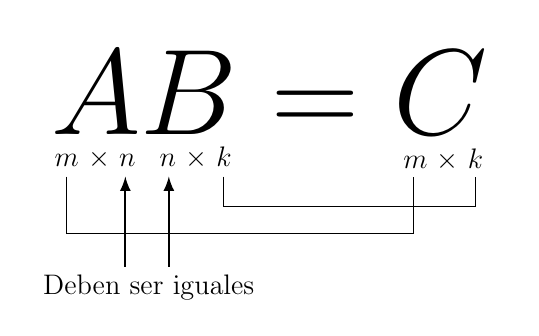
\begin{tikzpicture}[scale=0.85,transform shape]
            \begin{scope}[scale=3,transform shape]
                \node at (0,0) {\LARGE $AB = C$};
            \end{scope}
            
            \begin{scope}[xshift=-1.8cm]
                %\draw[ thick, <-,orange] (-0.15,0.25) .. controls (-0.25,0.8) and (-0.25,1.5) .. (1,1.5);
                
                %\node[right, orange] at (1,1.5) {\itshape No product symbol};
                \node[ ] at (-0.8,-1) {\large ${m}$ $\times$ $n$};
                \node[ ] at (0.7,-0.97) {\large $n$ $\times$ $k$};
                \node[ ] at (4.4,-1) {\large $m$ $\times$ $k$};
                
                \draw[thin] (1.11,-1.25)--(1.11,-1.7)--(4.88,-1.7)--(4.88,-1.25);
                \draw[thin] (-1.23,-1.25)--(-1.23,-2.1)--(3.96,-2.1)--(3.96,-1.25);
                
                \draw[thick, -latex] (-0.35,-2.6)--(-0.35,-1.25);
                \draw[thick, -latex] (0.3,-2.6)--(0.3,-1.25);
                \node at (0,-2.9) {\large Deben ser iguales};
            \end{scope}
        \end{tikzpicture}
    \end{center}
\end{observation}

\begin{example}
    En este ejemplo se muestra la forma en la cual se puede usar la multiplicación de matrices para modelar la manera en que se extiende una enfermedad contagiosa. Las enfermedades contagiosas son aquellas que se propagan de una persona a otra a través del contacto directo. Los ejemplos incluyen la gripe, el resfriado común y la COVID-19.
    
    Considere tres grupos de personas $X$, $Y$ y $Z$ con $4$, $6$ y $5$ elementos respectivamente como se muestra en la tabla \ref{tab:1}. Suponga que cuatro individuos han contraído esta enfermedad. Este grupo entra en contacto con seis personas de un segundo grupo. Estos contactos, llamados \textit{contactos directos}, se pueden representar por una matriz de $4 \times 6$. Consideremos la siguiente matriz para los grupos $X$ y $Y$:\sideTable[\label{tab:1}]{
    \centering
    \begin{tabular}{ll}
        \toprule
        \textbf{Grupo} & \textbf{Elementos} \\
        \midrule
        $X$ & $a_1$, $a_2$, $a_3$, $a_4$ \\
        $Y$ & $b_1$, $b_2$, $b_3$, $b_4$, $b_5$, $b_6$ \\
        $Z$ & $c_1$, $c_2$, $c_3$, $c_4$, $c_5$ \\
        \bottomrule
    \end{tabular}
    }
    $$A = \begin{bmatrix}
        0 & 1 & 0 & 0 & 1 & 0 \\
        1 & 0 & 0 & 1 & 0 & 1 \\
        0 & 0 & 0 & 1 & 1 & 0 \\
        1 & 0 & 0 & 0 & 0 & 1
    \end{bmatrix}$$
    En este caso se hace $a_{ij} = 1$ si la $i$-ésima persona del primer grupo entra en contacto con la $j$-ésima persona del segundo grupo. Por ejemplo, el $1$ en la posición $(2, 4)$ significa que la segunda persona del primer grupo (infectada) entró en contacto con la cuarta persona del segundo grupo. Ahora suponga que un tercer grupo de cinco personas tiene varios contactos directos con individuos del segundo grupo. Esto también se puede representar mediante una matriz.
    $$B = \begin{bmatrix}
        0 & 0 & 1 & 0 & 1 \\
        0 & 0 & 0 & 1 & 0 \\
        0 & 1 & 0 & 0 & 0 \\
        1 & 0 & 0 & 0 & 1 \\
        0 & 0 & 0 & 1 & 0 \\
        0 & 0 & 1 & 0 & 0
    \end{bmatrix}$$
    Observe que $b_{64} = 0$, lo que quiere decir que la sexta persona del segundo grupo no tiene contacto con la cuarta persona del tercer grupo.
    
    Los contactos \textit{indirectos} o de \textit{segundo orden} entre individuos del primero y tercer grupos se representan mediante la matriz de $4 \times 5$, $C = AB$. Para ver esto, observe que una persona del grupo $3$ puede quedar contagiada por alguien del grupo $2$, quien a su vez fue contagiada por alguien del grupo $1$. Por ejemplo, como $a_{24} = 1$ y $b_{45} = 1$ se ve que, indirectamente, la quinta persona del grupo $3$ tuvo contacto (a través de la cuarta persona del grupo $2$) con la segunda persona del grupo $1$. El número total de contactos indirectos entre la segunda persona del grupo $1$ y la quinta persona del grupo $3$ está dado por
    \begin{align*}
        c_{25} & = a_{21}b_{15} + a_{22}b_{25} + a_{23}b_{35} + a_{24}b_{45} + a_{25}b_{55} + a_{26}b_{65} \\
        & = 1 \cdot 1 + 0 \cdot 0 + 0 \cdot 0 + 1 \cdot 1 + 0 \cdot 0 + 1 \cdot 0 = 2
    \end{align*}
    Así pues,
    $$C = AB = \begin{bmatrix}
        0 & 0 & 0 & 2 & 0 \\
        1 & 0 & 2 & 0 & 2 \\
        1 & 0 & 0 & 1 & 1 \\
        0 & 0 & 2 & 0 & 1 
    \end{bmatrix}$$

    Observe que únicamente la segunda persona del grupo $3$ no tiene contactos indirectos con la enfermedad. La quinta persona de este grupo tiene $2 + 1 + 1 = 4$ contactos de segundo orden.
\end{example}

\begin{theorem}
    El producto de matrices es asociativo.
\end{theorem}

\begin{observation}
    El producto de matrices no es conmutativo. En efecto, sea $A$, $B \in \mathcal{M}_{2 \times 2}(\RR)$ con $A = \begin{bmatrix}
        1 & 1 \\
        0 & 1
    \end{bmatrix}$ y $B = \begin{bmatrix}
        2 & 1 \\
        1 & 1
    \end{bmatrix}$, entonces
    \begin{align*}
        AB & = \begin{bmatrix}
            1 & 1 \\
            0 & 1
        \end{bmatrix} \begin{bmatrix}
            2 & 1 \\
            1 & 1
        \end{bmatrix} \\
        & = \begin{bmatrix}
            3 & 2 \\
            1 & 1
        \end{bmatrix}
    \end{align*}
    y
    \begin{align*}
        BA & = \begin{bmatrix}
            2 & 1 \\
            1 & 1
        \end{bmatrix} \begin{bmatrix}
            1 & 1 \\
            0 & 1
        \end{bmatrix} \\
        & = \begin{bmatrix}
            2 & 3 \\
            1 & 2
        \end{bmatrix}
    \end{align*}
    Así que, en general $AB \neq BA$.
\end{observation}

\begin{notation}
    Si $A \in \mathcal{M}_{n \times n}(\RR)$ y $n \in \NN$, definimos $A^n$ como
    $$A^n = \underbrace{A A \cdots A}_{n-\text{veces}}$$
\end{notation}

\begin{definition}\label{def:matriz-idempotente}
    Sea $A \in \mathcal{M}_{n \times n}(\RR)$, decimos que $A$ es una matriz idempotente si $A^2=A$.
\end{definition}

\begin{example}
    Sea $A = \begin{bmatrix*}[r]
        -1 & 3 & 5 \\
        1 & -3 & -5 \\
        -1 & 3 & 5 \\
    \end{bmatrix*}$, entonces
    $$A^2 = \begin{bmatrix*}[r]
        -1 & 3 & 5 \\
        1 & -3 & -5 \\
        -1 & 3 & 5 \\
    \end{bmatrix*} \begin{bmatrix*}[r]
        -1 & 3 & 5 \\
        1 & -3 & -5 \\
        -1 & 3 & 5 \\
    \end{bmatrix*} = \begin{bmatrix*}[r]
        -1 & 3 & 5 \\
        1 & -3 & -5 \\
        -1 & 3 & 5 \\
    \end{bmatrix*} = A$$
    Por tanto, $A$ es idempotente.
\end{example}

\begin{definition}
    Sea $A \in \mathcal{M}_{n \times n}(\RR)$, decimos que $A$ es una matriz nilpotente si existe un entero positivo $p$ tal que $A^p=0$. El grado o índice de nilpotencia es el menor entero positivo $p$ tal que $A^p=0$.
\end{definition}

\begin{example}
    Sea $A = \begin{bmatrix*}[r]
        1 & 1 \\
        -1 & -1 \\
    \end{bmatrix*}$, entonces
    $$A^2 = \begin{bmatrix*}[r]
        1 & 1 \\
        -1 & -1 \\
    \end{bmatrix*} \begin{bmatrix*}[r]
        1 & 1 \\
        -1 & -1 \\
    \end{bmatrix*} = \begin{bmatrix*}[r]
        0 & 0 \\
        0 & 0 \\
    \end{bmatrix*}$$
    Por tanto, $A$ es nilpotente de índice de nilpotencia 2.
\end{example}

\begin{definition}
    La matriz identidad $I_n$ es una matriz de $n \times n$ cuyos elementos de la diagonal principal son iguales a $1$ y todos los demás son $0$. Esto es,
    $$I_n = \llparenthesis \delta_{ij} \rrparenthesis = \begin{cases}
        1 & \text{ si } i = j \\
        0 & \text{ si } i \neq j
    \end{cases}$$
\end{definition}

\begin{theorem}[Ley distributiva de la multiplicación de matrices]
    Si todas las sumas y todos los productos siguientes están definidos, entonces
    $$A(B + C) = AB + AC$$
    \demostracion
    Sea $A \in \mathcal{M}_{m \times p}(\RR)$ y sean $B$, $C \in \mathcal{M}_{p \times n}(\RR)$ con $A = \llparenthesis a_{ij} \rrparenthesis$, $B = \llparenthesis b_{kj} \rrparenthesis$, $C = \llparenthesis c_{kj} \rrparenthesis$. Así
    %{\small
    \begin{align*}
        A(B + C) & = \begin{bmatrix}
            a_{11} & a_{12} & \cdots & a_{1p}\\
            a_{21} & a_{22} & \cdots & a_{2p}\\
            \vdots &  & \ddots & \\
            a_{m1} & a_{m2} & \cdots & a_{mp}
        \end{bmatrix} \left( \begin{bmatrix}
            b_{11} & b_{12} & \cdots & b_{1n}\\
            b_{21} & b_{22} & \cdots & b_{2n}\\
            \vdots &  & \ddots & \\
            b_{p1} & b_{p2} & \cdots & b_{pn}
        \end{bmatrix} + \begin{bmatrix}
            c_{11} & c_{12} & \cdots & c_{1n}\\
            c_{21} & c_{22} & \cdots & c_{2n}\\
            \vdots &  & \ddots & \\
            c_{p1} & c_{p2} & \cdots & c_{pn}
        \end{bmatrix} \right) \\
        & = \begin{bmatrix}
            a_{11} & a_{12} & \cdots & a_{1p}\\
            a_{21} & a_{22} & \cdots & a_{2p}\\
            \vdots &  & \ddots & \\
            a_{m1} & a_{m2} & \cdots & a_{mp}
        \end{bmatrix} \begin{bmatrix}
            b_{11} + c_{11} & b_{12} + c_{12} & \cdots & b_{1n} + c_{1n}\\
            b_{21} + c_{21} & b_{22} + c_{22} & \cdots & b_{2n} + c_{2n}\\
            \vdots &  & \ddots & \\
            b_{p1} + c_{p1} & b_{p2} + c_{p2} & \cdots & b_{pn} + c_{pn}
        \end{bmatrix} \\
        & = \begin{bmatrix}
            \displaystyle\sum_{q=1}^{p} a_{1q}(b_{q1} + c_{q1}) & \displaystyle\sum_{q=1}^{p} a_{1q}(b_{q2} + c_{q2}) & \cdots & \displaystyle\sum_{q=1}^{p} a_{1q}(b_{qn} + c_{qn}) \\
            \displaystyle\sum_{q=1}^{p} a_{2q}(b_{q1} + c_{q1}) & \displaystyle\sum_{q=1}^{p} a_{2q}(b_{q2} + c_{q2}) & \cdots & \displaystyle\sum_{q=1}^{p} a_{2q}(b_{qn} + c_{qn}) \\
            \vdots & & \ddots & \\
            \displaystyle\sum_{q=1}^{p} a_{mq}(b_{q1} + c_{q1}) & \displaystyle\sum_{q=1}^{p} a_{mq}(b_{q2} + c_{q2}) & \cdots & \displaystyle\sum_{q=1}^{p} a_{mq}(b_{qn} + c_{qn})
        \end{bmatrix} \\
        & = \begin{bmatrix}
            \displaystyle\sum_{q=1}^{p} a_{1q}b_{q1} + \displaystyle\sum_{q=1}^{p} a_{1q}c_{q1} & \displaystyle\sum_{q=1}^{p} a_{1q}b_{q2} + \displaystyle\sum_{q=1}^{p} a_{1q}c_{q2} & \cdots & \displaystyle\sum_{q=1}^{p} a_{1q}b_{qn} + \displaystyle\sum_{q=1}^{p} a_{1q}c_{qn} \\
            \displaystyle\sum_{q=1}^{p} a_{2q}b_{q1} + \displaystyle\sum_{q=1}^{p} a_{2q}c_{q1} & \displaystyle\sum_{q=1}^{p} a_{2q}b_{q2} + \displaystyle\sum_{q=1}^{p} a_{2q}c_{q2} & \cdots & \displaystyle\sum_{q=1}^{p} a_{2q}b_{qn} + \displaystyle\sum_{q=1}^{p} a_{2q}c_{qn} \\
            \vdots & & \ddots & \\
            \displaystyle\sum_{q=1}^{p} a_{mq}b_{q1} + \displaystyle\sum_{q=1}^{p} a_{mq}c_{q1} & \displaystyle\sum_{q=1}^{p} a_{mq}b_{q2} + \displaystyle\sum_{q=1}^{p} a_{mq}c_{q2} & \cdots & \displaystyle\sum_{q=1}^{p} a_{mq}b_{qn} + \displaystyle\sum_{q=1}^{p} a_{mq}c_{qn}
        \end{bmatrix} \\
        & = \begin{bmatrix}
            \displaystyle\sum_{q=1}^{p} a_{1q}b_{q1} & \displaystyle\sum_{q=1}^{p} a_{1q}b_{q2} & \cdots & \displaystyle\sum_{q=1}^{p} a_{1q}b_{qn} \\
            \displaystyle\sum_{q=1}^{p} a_{2q}b_{q1} & \displaystyle\sum_{q=1}^{p} a_{2q}b_{q2} & \cdots & \displaystyle\sum_{q=1}^{p} a_{2q}b_{qn} \\
            \vdots & & \ddots & \\
            \displaystyle\sum_{q=1}^{p} a_{mq}b_{q1} & \displaystyle\sum_{q=1}^{p} a_{mq}b_{q2} & \cdots & \displaystyle\sum_{q=1}^{p} a_{mq}b_{qn} 
        \end{bmatrix} + \begin{bmatrix}
            \displaystyle\sum_{q=1}^{p} a_{1q}c_{q1} & \displaystyle\sum_{q=1}^{p} a_{1q}c_{q2} & \cdots & \displaystyle\sum_{q=1}^{p} a_{1q}c_{qn} \\
            \displaystyle\sum_{q=1}^{p} a_{2q}c_{q1} & \displaystyle\sum_{q=1}^{p} a_{2q}c_{q2} & \cdots & \displaystyle\sum_{q=1}^{p} a_{2q}c_{qn} \\
            \vdots & & \ddots & \\
            \displaystyle\sum_{q=1}^{p} a_{mq}c_{q1} & \displaystyle\sum_{q=1}^{p} a_{mq}c_{q2} & \cdots & \displaystyle\sum_{q=1}^{p} a_{mq}c_{qn}
        \end{bmatrix} \\
        & = AB + AC
    \end{align*}
    %}
\end{theorem}

\begin{definition}
    Sea $A \in \mathcal{M}_{n\times n} (\RR)$ y sea $f(x) \in P_n(x)$, con
    $$f(x)=a_0 + a_1 x+ \cdots +a_m x^m$$
    Definimos a $f(A)$ como:
    $$f(A)=a_0 I_n +a_1 A+\cdots +a_m A^m$$
\end{definition}

\begin{example}
    Si $f(x) = x^2 -5x +2$ y $A = \begin{bmatrix}
        2 & 0 \\
        4 & 5 \\
    \end{bmatrix}$, entonces:
    $$f(A) = \begin{bmatrix}
        2 & 0 \\
        4 & 5 \\
    \end{bmatrix} \begin{bmatrix}
        2 & 0 \\
        4 & 5 \\
    \end{bmatrix} -5 \begin{bmatrix}
        2 & 0 \\
        4 & 5 \\
    \end{bmatrix} +2 \begin{bmatrix}
        1 & 0 \\
        0 & 1 \\
    \end{bmatrix} = \begin{bmatrix*}[r]
        -4 & 0 \\
        8 & 2 \\
    \end{bmatrix*}$$
\end{example}

\begin{definition}
    Sea $A = \llparenthesis a_{ij} \rrparenthesis \in \mathcal{M}_{m \times n}(\RR)$, se define la matriz transpuesta de $A$, denotada por $A^T$ donde $A^T \in \mathcal{M}_{n \times m}(\RR)$, como sigue: Si
    $$A = \begin{bmatrix}
        a_{11} & a_{12} & \cdots & a_{1n}\\
        a_{21} & a_{22} & \cdots & a_{2n}\\
        \vdots &  & \ddots & \\
        a_{m1} & a_{m2} & \cdots & a_{mn}
    \end{bmatrix}$$
    entonces
    $$A^T = \llparenthesis a_{ji} \rrparenthesis = \begin{bmatrix}
        a_{11} & a_{21} & \cdots & a_{m1}\\
        a_{12} & a_{22} & \cdots & a_{m2}\\
        \vdots &  & \ddots & \\
        a_{1n} & a_{2n} & \cdots & a_{mn}
    \end{bmatrix}$$
\end{definition}

\begin{example}
    Un torneo de Tenis se puede organizar de la siguiente manera. Cada uno de los $n$ tenistas juega contra todas los demás y se registran los resultados en una matriz $R = \llparenthesis r_{ij} \rrparenthesis \in \mathcal{M}_{n \times n}(\RR)$ como sigue:
    $$r_{ij} = \begin{cases}
        1, & \text{ si el jugador $i$ le gana al $j$} \\
        0, & \text{ si el jugador $i$ pierde contra el $j$} \\
        0, & \text{ si $i = j$}
    \end{cases}$$
    Se asigna al tenista $i$ la calificación siguiente:
    \begin{equation}
        S_i = \sum_{j=1}^{n} r_{ij} + \frac{1}{2} \sum_{j=1}^{n} \left( R^{2} \right)_{ij} \label{ec28}
    \end{equation}
    Para un torneo de $n = 4$ tenistas, tenemos
    $$R = \begin{bmatrix}
        0 & 1 & 0 & 0 \\
        0 & 0 & 1 & 1 \\
        1 & 0 & 0 & 0 \\
        1 & 0 & 1 & 0
    \end{bmatrix} = \llparenthesis r_{ij} \rrparenthesis$$
    Para clasificar a los jugadores, primero calculemos $R^{2}$ como sigue:
    $$R^{2} = \begin{bmatrix}
        0 & 1 & 0 & 0 \\
        0 & 0 & 1 & 1 \\
        1 & 0 & 0 & 0 \\
        1 & 0 & 1 & 0
    \end{bmatrix} \begin{bmatrix}
        0 & 1 & 0 & 0 \\
        0 & 0 & 1 & 1 \\
        1 & 0 & 0 & 0 \\
        1 & 0 & 1 & 0
    \end{bmatrix} = \begin{bmatrix}
        0 & 0 & 1 & 1 \\
        2 & 0 & 1 & 0 \\
        0 & 1 & 0 & 0 \\
        1 & 1 & 0 & 0
    \end{bmatrix}$$
    Así, utilizando la ecuación \eqref{ec28}, obtenemos:
    \begin{align*}
        S_1 & = 1 + \frac{1}{2} (2) & S_2 & = 2 + \frac{1}{2} (3) & S_3 & = 1 + \frac{1}{2} (1) & S_4 & = 2 + \frac{1}{2} (2) \\
        & = 2 & & = \frac{7}{2} & & = \frac{3}{2} & & = 3
    \end{align*}
    Por tanto, $S_1 = 2$, $\displaystyle S_2 = \frac{7}{2}$, $\displaystyle S_3 = \frac{3}{2}$ y $S_4 = 4$, y además
    $$S_3 < S_1 < S_4 < S_2.$$
\end{example}

\begin{definition}
    Sea $A \in \mathcal{M}_{n \times n}(\RR)$. Si $A^T = A$, entonces decimos que la matriz $A$ es simétrica.
\end{definition}

\newpage

\begin{example}
    Sea $A = \begin{bmatrix}
        1 & 3 \\
        3 & 1
    \end{bmatrix}$. Notemos que $A^T = A$, por lo que $A$ es simétrica.
\end{example}

\begin{definition}\label{matriz-antisimetrica}
    Sea $A \in \mathcal{M}_{n \times n}(\RR)$. Si $A^T = -A$, entonces decimos que la matriz $A$ es antisimétrica.
\end{definition}

\begin{theorem}\label{theo:matrixtranspu}
    Sea $A$, $B \in \mathcal{M}_{n \times n}(\RR)$, entonces
    $$(AB)^T = B^TA^T$$
    \demostracion
    Sea
    $$A = \begin{bmatrix}
        a_{11} & a_{12} & \cdots & a_{1n}\\
        a_{21} & a_{22} & \cdots & a_{2n}\\
        \vdots &  & \ddots & \\
        a_{n1} & a_{n2} & \cdots & a_{nn}
    \end{bmatrix}$$
    entonces
    $$A^T = \begin{bmatrix}
        a_{11} & a_{21} & \cdots & a_{n1}\\
        a_{12} & a_{22} & \cdots & a_{n2}\\
        \vdots &  & \ddots & \\
        a_{1n} & a_{2n} & \cdots & a_{nn}
    \end{bmatrix}$$
    Análogamente, sea
    $$B = \begin{bmatrix}
        b_{11} & b_{12} & \cdots & b_{1n}\\
        b_{21} & b_{22} & \cdots & b_{2n}\\
        \vdots &  & \ddots & \\
        b_{n1} & b_{n2} & \cdots & b_{nn}
    \end{bmatrix}$$
    entonces
    $$B^T = \begin{bmatrix}
        b_{11} & b_{21} & \cdots & b_{n1}\\
        b_{12} & b_{22} & \cdots & b_{n2}\\
        \vdots &  & \ddots & \\
        b_{1n} & b_{2n} & \cdots & b_{nn}
    \end{bmatrix}$$
    Ahora
    $$AB = \begin{bmatrix}
        \displaystyle\sum_{q=1}^{n} a_{1q}b_{q1} & \displaystyle\sum_{q=1}^{n} a_{1q}b_{q2} & \cdots & \displaystyle\sum_{q=1}^{n} a_{1q}b_{qn} \\
        \displaystyle\sum_{q=1}^{n} a_{2q}b_{q1} & \displaystyle\sum_{q=1}^{n} a_{2q}b_{q2} & \cdots & \displaystyle\sum_{q=1}^{n} a_{2q}b_{qn} \\
        \vdots & & \ddots & \\
        \displaystyle\sum_{q=1}^{n} a_{nq}b_{q1} & \displaystyle\sum_{q=1}^{n} a_{nq}b_{q2} & \cdots & \displaystyle\sum_{q=1}^{n} a_{nq}b_{qn}
    \end{bmatrix}$$
    Por otra parte
    $$B^T A^T = \begin{bmatrix}
        \displaystyle\sum_{q=1}^{n} a_{1q}b_{q1} & \displaystyle\sum_{q=1}^{n} a_{2q}b_{q1} & \cdots & \displaystyle\sum_{q=1}^{n} a_{nq}b_{q1} \\
        \displaystyle\sum_{q=1}^{n} a_{1q}b_{q2} & \displaystyle\sum_{q=1}^{n} a_{2q}b_{q2} & \cdots & \displaystyle\sum_{q=1}^{n} a_{nq}b_{q2} \\
        \vdots & & \ddots & \\
        \displaystyle\sum_{q=1}^{n} a_{1q}b_{qn} & \displaystyle\sum_{q=1}^{n} a_{2q}b_{qn} & \cdots & \displaystyle\sum_{q=1}^{n} a_{nq}b_{qn} 
    \end{bmatrix} = (AB)^T$$
\end{theorem}

\begin{proposition}
    Sean $A$, $B \in \mathcal{M}_{n \times n}(\RR)$ y sea $\alpha \in \RR$, entonces
    \begin{enumerate}[label=\roman*.]
        \item $\left(A^T\right)^T = A$.
        \item $(A + B)^T = A^T + B^T$
        \item $(\alpha A)^T = \alpha A^T$
    \end{enumerate}
    \demostracion Se dejan como ejercicio al lector.
\end{proposition}

\begin{definition}
    Sea $A \in \mathcal{M}_{n \times n}(\RR)$, decimos que $A$ es una matriz diagonal si todas sus entradas fuera de la diagonal son cero, es decir, $\llparenthesis a_{ij} \rrparenthesis = 0$, para toda $i \neq j$. Si $\llparenthesis a_{ij} \rrparenthesis = a_{ij}$, entonces escribiremos $$A = \operatorname{diag} \left\lbrace a_{11}, \dots, a_{nn} \right\rbrace$$
\end{definition}

\begin{example}
    Sea
    $$A = \begin{bmatrix*}[r]
        -1 & 0 & 0 \\
        0 & -6 & 0 \\
        0 & 0 & -9 \\
    \end{bmatrix*}$$
    entonces $A = \operatorname{diag} \{ -1, -6, -9 \}$.
\end{example}

\begin{proposition}
    Sean $A$, $B$ matrices diagonales y sea $\alpha \in \RR$, entonces
    \begin{enumerate}[label=\roman*.]
        \item $A+B$ es diagonal.
        \item $AB$ es diagonal.
        \item $\alpha A$ es diagonal.
    \end{enumerate}
    \demostracion Se dejan como ejercicio al lector.
\end{proposition}

\begin{definition}
    Sea $A \in \mathcal{M}_{n \times n}(\RR)$, decimos que $A$ es una matriz triangular superior si todas las entradas bajo la diagonal son cero, es decir, $\llparenthesis a_{ij} \rrparenthesis = 0$, para toda $i>j$.
\end{definition}

\begin{example}
    Un ejemplo de una matriz triangular superior es:
    \begin{center}
        \begin{tikzpicture}[
        Matrix/.style={
        matrix of nodes,
        text height=1.75ex,
        text depth=0.525ex,
        text width=2.275ex,
        align=center,
        left delimiter={[},
        right delimiter={]},
        column sep=0pt,
        row sep=0pt,
        nodes in empty cells,},
        DA/.style={
        fill=gray!20,
        dash pattern=on 3pt off 3pt,
        line width=0.7pt,
        rounded corners=5pt,}
        ]
        
        \matrix[Matrix] at (0,0) (M){
            $1$ & $6$ & $1$ \\
            $0$ & $2$ & $7$ \\
            $0$ & $0$ & $9$ \\
        };
        
        \begin{scope}[on background layer]
            \draw[DA](M-1-1.north west)
            -| (M-3-3.south east)
            -- (M-3-3.south west)
            |- (M-2-2.south west)
            |- (M-1-1.south west)
            -- cycle;
        \end{scope}
        \end{tikzpicture}
    \end{center}
\end{example}

\begin{proposition}
    Sean $A$, $B$ matrices triangulares superiores y sea $\alpha \in \RR$, entonces
    \begin{enumerate}[label=\roman*.]
        \item $A+B$ es triangular superior.
        \item $AB$ es triangular superior.
        \item $\alpha A$ es triangular superior.
    \end{enumerate}
    \demostracion Se dejan como ejercicio al lector.
\end{proposition}

\begin{definition}
    Sea $A \in \mathcal{M}_{n \times n}(\RR)$, decimos que $A$ es una matriz triangular inferior si todas las entradas sobre la diagonal son cero, es decir, $\llparenthesis a_{ij} \rrparenthesis = 0$, para toda $i<j$.
\end{definition}

\begin{example}
    Un ejemplo de una matriz triangular inferior es:
    \begin{center}
        \begin{tikzpicture}[scale=0.9,
        Matrix/.style={
        matrix of nodes,
        text height=1.75ex,
        text depth=0.525ex,
        text width=2.275ex,
        align=center,
        left delimiter={[},
        right delimiter={]},
        column sep=0pt,
        row sep=0pt,
        nodes in empty cells,},
        DA/.style={
        fill=gray!20,
        dash pattern=on 3pt off 3pt,
        line width=0.7pt,
        rounded corners=5pt,}
        ]
        
        \matrix[Matrix] at (0,0) (M1){
            $6$ & $0$ & $0$ \\
            $4$ & $3$ & $0$ \\
            $8$ & $5$ & $1$ \\
        };
        
        \begin{scope}[on background layer]
            \draw[DA](M1-1-1.north)
            -| (M1-1-1.south east)
            -| (M1-2-2.south east)
            -| (M1-3-3.south east)
            -| (M1-1-1.west)
            |- (M1-1-1.north);
        \end{scope}
        \end{tikzpicture}
    \end{center}
\end{example}

\newpage

\begin{proposition}
    Sean $A$, $B$ matrices triangulares inferiores y sea $\alpha \in \RR$, entonces
    \begin{enumerate}[label=\roman*.]
        \item $A+B$ es triangular inferior.
        \item $AB$ es triangular inferior.
        \item $\alpha A$ es triangular inferior.
    \end{enumerate}
    \demostracion Se dejan como ejercicio al lector.
\end{proposition}

\section{Sistemas de ecuaciones}

\begin{definition}\label{definicion:JSJJNDJUDUDJNDN}
    Sea $A \in \mathcal{M}_{n \times n}(\RR)$ y $\mathbb{x} \in \RR[n]$, siendo
    $$A = \begin{bmatrix}
        a_{11} & a_{12} & \cdots & a_{1n}\\
        a_{21} & a_{22} & \cdots & a_{2n}\\
        \vdots &  & \ddots & \\
        a_{m1} & a_{m2} & \cdots & a_{mn}
    \end{bmatrix} \quad \text{y} \quad \mathbb{x} = \begin{bmatrix}
        x_1 \\
        x_2 \\
        \vdots \\
        x_n
    \end{bmatrix}$$
    Se define el producto de la matriz $A$ con el vector $\mathbb{x}$ como:
    \begin{align*}
        A \mathbb{x} = \begin{bmatrix}
            a_{11} & a_{12} & \cdots & a_{1n}\\
            a_{21} & a_{22} & \cdots & a_{2n}\\
            \vdots &  & \ddots & \\
            a_{m1} & a_{m2} & \cdots & a_{mn}
        \end{bmatrix} \begin{bmatrix}
            x_1 \\
            x_2 \\
            \vdots \\
            x_n
        \end{bmatrix} = \begin{bmatrix}
            a_{11}x_1 + a_{12}x_2 + \cdots + a_{1n}x_n \\
            a_{21}x_1 + a_{22}x_2 + \cdots + a_{2n}x_n \\
            \vdots \\
            a_{m1}x_1 + a_{m2}x_2 + \cdots + a_{mn}x_n
        \end{bmatrix}
    \end{align*}
\end{definition}

\begin{definition}
    Si $A\mathbb{x} = \mathbb{b}$, obtenemos
    \begin{equation}
        \left. \begin{array}{rl}
            a_{11}x_1 + a_{12}x_2 + \cdots + a_{1n}x_n = & \!\!\!\! b_1 \\
            a_{21}x_1 + a_{22}x_2 + \cdots + a_{2n}x_n = & \!\!\!\! b_2 \\
            \vdots \hspace{1cm}  \\
            a_{m1}x_1 + a_{m2}x_2 + \cdots + a_{mn}x_n = & \!\!\!\! b_m
        \end{array} \!\!\right\} \label{ec29}
    \end{equation}
    A la expresión \eqref{ec29} se le llamará \textbf{sistema de ecuaciones lineales} (SEL) de $m$ ecuaciones con $n$ incógnitas. Además, si $\mathbb{b} = \mathbb{0}$, obtenemos
    \begin{equation*}
        \left. \begin{array}{rl}
            a_{11}x_1 + a_{12}x_2 + \cdots + a_{1n}x_n = & \!\!\!\! 0 \\
            a_{21}x_1 + a_{22}x_2 + \cdots + a_{2n}x_n = & \!\!\!\! 0 \\
            \vdots \hspace{1cm}  \\
            a_{m1}x_1 + a_{m2}x_2 + \cdots + a_{mn}x_n = & \!\!\!\! 0
        \end{array} \!\!\right\}
    \end{equation*}
    A esta expresión se le llamará sistema homogéneo.
\end{definition}

\begin{observation}
    Una solución para el sistema homogéneo es cuando $x_1 = x_2 = \cdots = x_n = 0$ y es conocida como solución trivial.
\end{observation}
\marginElement{
\begin{center}
    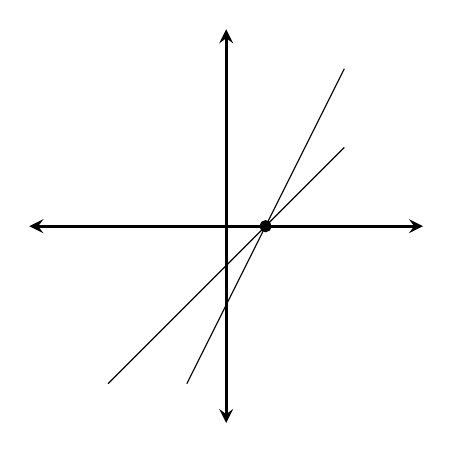
\begin{tikzpicture}
        \draw[black,stealth-stealth,very thick] (0,0) -- (5,0);
        \draw[black,stealth-stealth,very thick] (2.5,-2.5) -- (2.5,2.5);
        \draw (1,-2) -- (4,1);
        \draw (2,-2) -- (4,2);
        \filldraw (3,0) circle (2pt); 
    \end{tikzpicture}
    \textbf{i.} Sistemas con única solución
\end{center}
~\vspace{-0.5cm}
\begin{center}
    \begin{tikzpicture}
        \draw[black,stealth-stealth,very thick] (0,0) -- (5,0);
        \draw[black,stealth-stealth,very thick] (2.5,-2.5) -- (2.5,2.5);
        \draw[thick] (1,-2) -- (4,2);
        \draw (1,-2) -- (4,2);
    \end{tikzpicture}
    \textbf{ii.} Sistemas con infinitas soluciones
\end{center}
~\vspace{-0.5cm}
\begin{center}
    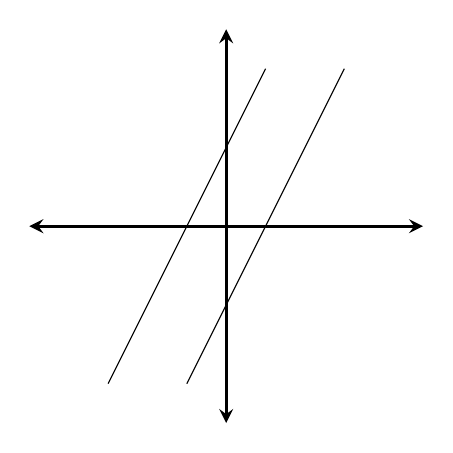
\begin{tikzpicture}
        \draw[black,stealth-stealth,very thick] (12,0) -- (17,0);
        \draw[black,stealth-stealth,very thick] (14.5,-2.5) -- (14.5,2.5);
        \draw (13,-2) -- (15,2);
        \draw (14,-2) -- (16,2);
    \end{tikzpicture}
    \textbf{iii.} Sistemas sin solución
\end{center}
\captionsetup*[figure]{font={footnotesize},hypcap=false}%
\captionof{figure}{Representación de los posibles casos del conjunto solución de un SEL $2 \times 2$}\label{JWISIKSJSKISOOKKOOOOIUKKSK}
}

Consideremos el siguiente sistema de dos ecuaciones lineales con dos incógnitas $x_1$, $x_2$:
$$\left. \begin{array}{rl}
    a_{11}x_1+a_{12}x_2 = & \!\!\!\! b_1 \\ 
    a_{21}x_1+a_{22}x_2 = & \!\!\!\! b_2 \\
\end{array} \!\!\right\}$$
donde $a_{11}$, $a_{12}$, $a_{21}$, $a_{22}$, $b_1$, $b_2$ son números dados. Notemos que cada una de estas ecuaciones corresponde a una recta. Cualquier par ordenado de números reales $(x_1, x_2)$ que satisface dicho sistema se denomina como solución. Notemos que en este sistema existen tres posibles casos: cuando existe una única solución, infinitas soluciones o el conjunto solución es el vacío. Vea la figura \ref{JWISIKSJSKISOOKKOOOOIUKKSK}.
\newpage
\marginElement{
\begin{center}
    \tdplotsetmaincoords{70}{110}
    \begin{tikzpicture}[tdplot_main_coords,scale=0.65]
        \begin{scope}
            \draw[fill=gray!50,opacity=0.3] (0,0,0) -- (0,-3,-1) -- (0,-3,-3) -- (0,0,-3) -- cycle;
            \draw[fill=gray!60,opacity=0.3] (-3,-3,-1) -- (-3,0,0) -- (3,0,0) -- (3,-3,-1) -- cycle;
            \draw[fill=gray!50,opacity=0.3] (0,-3,3) -- (0,0,3) -- (0,0,0) -- (0,-3,-1) -- cycle;
            \draw[fill=gray!80,opacity=0.4] (-3,0,-3) -- (-3,0,3) -- (3,0,3) -- (3,0,-3) -- cycle;
            \draw[fill=gray!50,opacity=0.3] (0,0,0) -- (0,3,1) -- (0,3,-3) -- (0,0,-3) -- cycle;
            \draw[fill=gray!60,opacity=0.3] (-3,0,0) -- (-3,3,1) -- (3,3,1) -- (3,0,0) -- cycle;
            \draw[fill=gray!50,opacity=0.3] (0,0,0) -- (0,0,3) -- (0,3,3) -- (0,3,1) -- cycle;
            \filldraw (0,0,0) circle(4pt);
        \end{scope}
    \end{tikzpicture}
    \\ \textbf{i.} Sistemas con única solución
\end{center}
~\vspace{-0.5cm}
\begin{center}
    \tdplotsetmaincoords{70}{110}
    \begin{tikzpicture}[tdplot_main_coords,scale=0.65]
        \begin{scope}[xshift=8cm]
            \draw[fill=gray!50,opacity=0.3] (-3,0,0) -- (-3,-1,-3) -- (3,-1,-3) -- (3,0,0) -- cycle;
            \draw[fill=gray!60,opacity=0.3] (-3,-3,-1) -- (-3,0,0) -- (3,0,0) -- (3,-3,-1) -- cycle;
            \draw[fill=gray!80,opacity=0.4] (-3,0,-3) -- (-3,0,3) -- (3,0,3) -- (3,0,-3) -- cycle;
            \draw[fill=gray!60,opacity=0.3] (-3,0,0) -- (-3,3,1) -- (3,3,1) -- (3,0,0) -- cycle;
            \draw[fill=gray!50,opacity=0.3] (-3,1,3) -- (-3,0,0) -- (3,0,0) -- (3,1,3) -- cycle;
            \draw[thick, dashed, black](-3,0,0)--(3,0,0); 
        \end{scope}
    \end{tikzpicture}
    \\ \textbf{ii.} Sistemas con infinitas soluciones
\end{center}
~\vspace{-0.5cm}
\begin{center}
    \tdplotsetmaincoords{70}{110}
    \begin{tikzpicture}[tdplot_main_coords,scale=0.65]
        \draw[dash pattern=on 3pt off 3pt] (-3,-3,0) -- (-3,-3,5);
        \draw[fill=gray!50,opacity=0.3] (-3,-3,0) -- (-3,3,0) -- (3,3,0) -- (3,-3,0) -- cycle;
        \draw[fill=gray!70,opacity=0.35] (-3,-3,2.5) -- (-3,3,2.5) -- (3,3,2.5) -- (3,-3,2.5) -- cycle;
        \draw[fill=gray!90,opacity=0.4] (-3,-3,5) -- (-3,3,5) -- (3,3,5) -- (3,-3,5) -- cycle;
        \draw[dash pattern=on 3pt off 3pt] (-3,3,0) -- (-3,3,5);
        \draw[dash pattern=on 3pt off 3pt] (3,3,0) -- (3,3,5);
        \draw[dash pattern=on 3pt off 3pt] (3,-3,0) -- (3,-3,5);
    \end{tikzpicture}
    \,\\
    \tdplotsetmaincoords{80}{93}
    \begin{tikzpicture}[tdplot_main_coords,scale=0.8]
        \begin{scope}[xshift=16cm]
            \draw[fill=gray!50,opacity=0.3] (-3,-1,2) -- (-3,2,-2) -- (3,2,-2) -- (3,-1,2) -- cycle;
            \draw[fill=gray!80,opacity=0.4] (-3,1,2) -- (-3,-2,-2) -- (3,-2,-2) -- (3,1,2) -- cycle;
            \draw[fill=gray!60,opacity=0.3] (-3,-3,-1)--(-3,3,-1)--(3,3,-1)--(3,-3,-1) -- cycle;
            \draw[dashed,thick](-3,-1.25,-1)--(3,-1.25,-1);
            \draw[dashed,thick](-3,1.25,-1)--(3,1.25,-1);
            \draw[dashed,thick](-2.7,0,0.75)--(3,0,0.75);
            \draw[thin](-3,-1.25,-1)--(3,-1.25,-1);
            \draw[thin](-3,1.25,-1)--(3,1.25,-1);
            \draw[thin](-2.7,0,0.75)--(3,0,0.75);
        \end{scope}
    \end{tikzpicture}
    \\ \textbf{iii.} Sistemas sin solución
\end{center}
\captionsetup*[figure]{font={footnotesize},hypcap=false}%
\captionof{figure}{Representación de los posibles casos del conjunto solución de un SEL $3 \times 3$}\label{KSKJSJSJJJJSJSJJSDDDD}
}

Ahora, consideremos el siguiente sistema de tres ecuaciones lineales con tres incógnitas $x_1$, $x_2$, $x_3$:
$$\left. \begin{array}{rl}
    a_{11}x_1+a_{12}x_2+a_{13}x_3 = & \!\!\!\! b_1 \\ 
    a_{21}x_1+a_{22}x_2+a_{23}x_3 = & \!\!\!\! b_2 \\ 
    a_{31}x_1+a_{32}x_2+a_{33}x_3 = & \!\!\!\! b_3
\end{array} \!\!\right\}$$
donde $a_{11}$, $a_{12}$, $a_{13}$, $a_{21}$, $a_{22}$, $a_{23}$, $a_{31}$, $a_{32}$, $a_{33}$, $b_1$, $b_2$, $b_3$ son números dados. Notemos que cada una de estas ecuaciones corresponde a un plano. Cualquier terna de números reales $(x_1, x_2, x_3)$ que satisface dicho sistema se denomina como solución. De manera análoga respecto al SEL $2 \times 2$ anterior, en este sistema existen tres posibles casos: cuando existe una única solución, infinitas soluciones o el conjunto solución es el vacío. Es difícil dibujar con exactitud los planos en distintos casos, pero se pueden reducir como se muestra en la figura \ref{KSKJSJSJJJJSJSJJSDDDD}.

\begin{observation}
    Observemos que en la definición \ref{definicion:JSJJNDJUDUDJNDN} se puso a $\mathbb{x}$ como una matriz de tamaño $n \times 1$, cuando al principio de dicha definición se dijo que pertenecía a $\RR[n]$. Aunque pueda parecer un error, no es así, pues $\mathbb{x}$ se puede representar de ambas maneras, sea como vector o como matriz de tamaño $n \times 1$. Así que si $\mathbb{x} \in \RR[n]$, entonces $\mathbb{x} \in \mathcal{M}_{n \times 1}(\RR)$. Cuando consideremos a $\mathbb{x} \in \mathcal{M}_{n \times 1}(\RR)$, escribiremos a $\mathbb{x}$ como:
    $$\mathbb{x} = \begin{bmatrix}
        x_1 \\
        x_2 \\
        \vdots \\
        x_n
    \end{bmatrix}$$
    en vez de
    $$\mathbb{x} = \begin{pmatrix}
        x_1 \\
        x_2 \\
        \vdots \\
        x_n
    \end{pmatrix}$$
    Esto nos será de gran ayuda para entender de mejor manera los sistemas de ecuaciones lineales y no confundirnos con la notación.
\end{observation}

\section{Núcleo e imagen de una matriz}

\begin{definition}
    Sea $A \in \matrizmn$, se define el espacio nulo de $A$, denotado por $\mathcal{N}_A$, como:
    $$\mathcal{N}_A = \left\{ \mathbb{x} \in \RR[n] \mid A\mathbb{x} = \mathbb{0} \in \RR[m] \right\}$$
    Al espacio nulo de $A$ también de le llama kernel de $A$, o bien, núcleo de $A$.
\end{definition}

\begin{proposition}
    $\mathcal{N}_A$ es un subespacio de $\RR[n]$. \\
    \demostracion Basta probar que $\mathcal{N}_A$ cumple (i) y (ii) del teorema \ref{theorem:JAJSUJGBUHBOSOIOOSK}. Así pues:
    \begin{enumerate}[label=\roman*)]
        \item Sean $\mathbb{x}$, $\mathbb{y} \in \mathcal{N}_A$, entonces
        \begin{equation*}
            A\mathbb{x} = \mathbb{0} \quad \text{y} \quad A\mathbb{y} = \mathbb{0} \label{ec30}
        \end{equation*}
        Ahora
        \begin{align*}
            A(\mathbb{x}+\mathbb{y}) & = A \mathbb{x} + A \mathbb{y} \\
            & = \mathbb{0} + \mathbb{0} = \mathbb{0}
        \end{align*}
        Entonces $\mathbb{x} + \mathbb{y} \in \mathcal{N}_A$. Por tanto, se cumple la propiedad de cerradura para la suma.\newpage
        \item Sea $\alpha \in \RR$, veamos que $\alpha \mathbb{x} \in \mathcal{N}_A$. Así
        \begin{align*}
            A(\alpha \cdot \mathbb{x}) & = \begin{bmatrix}
                a_{11} & a_{12} & \cdots & a_{1n}\\
                a_{21} & a_{22} & \cdots & a_{2n}\\
                \vdots &  & \ddots & \\
                a_{m1} & a_{m2} & \cdots & a_{mn}
            \end{bmatrix} \begin{bmatrix}
                \alpha x_1 \\
                \alpha x_2 \\
                \vdots \\
                \alpha x_n
            \end{bmatrix} \\
            & = \begin{bmatrix}
                a_{11}\alpha x_1 + a_{12}\alpha x_2 + \cdots + a_{1n}\alpha x_n \\
                a_{21}\alpha x_1 + a_{22}\alpha x_2 + \cdots + a_{2n}\alpha x_n \\
                \vdots \\
                a_{m1}\alpha x_1 + a_{m2}\alpha x_2 + \cdots + a_{mn}\alpha x_n
            \end{bmatrix} \\
            & = \begin{bmatrix}
                \alpha \left( a_{11}x_1 + a_{12}x_2 + \cdots + a_{1n}x_n \right) \\
                \alpha \left( a_{21}x_1 + a_{22}x_2 + \cdots + a_{2n}x_n \right) \\
                \vdots \\
                \alpha \left( a_{m1}x_1 + a_{m2}x_2 + \cdots + a_{mn}x_n \right)
            \end{bmatrix} \\
            & = \alpha A \mathbb{x} \\
            & = \alpha \cdot \mathbb{0} = \mathbb{0}
        \end{align*}
        Entonces $\alpha \mathbb{x} \in \mathcal{N}_A$. Por tanto, se cumple la propiedad de cerradura para la multiplicación de un escalar por un vector.
    \end{enumerate}
    De (i) y (ii), se sigue que $\mathcal{N}_A$ es subespacio de $\RR[n]$.
\end{proposition}

\begin{definition}
    Llamaremos nulidad de $A$, denotada por $\nu(A)$, a la $\Dim(\mathcal{N}_A)$, es decir
    $$\nu(A) = \Dim(\mathcal{N}_A)$$
\end{definition}

\begin{example}
    Sea $A = \begin{bmatrix*}[r]
        1 & 2 & -1 \\
        2 & -1 & 3
    \end{bmatrix*} \in \mathcal{M}_{2 \times 3}(\RR)$, determine $\mathcal{N}_A$. \\
    \solucion Por definición,
    \begin{align*}
        \mathcal{N}_A & = \left\{ \mathbb{x} \in \RR[3] \mid A\mathbb{x} = \mathbb{0} \right\} \\
        & = \left\{ \begin{pmatrix}
            x_1 \\
            x_2 \\
            x_3
        \end{pmatrix} \mid \begin{bmatrix*}[r]
            1 & 2 & -1 \\
            2 & -1 & 3
        \end{bmatrix*} \begin{bmatrix}
            x_1 \\
            x_2 \\
            x_3
        \end{bmatrix} = \begin{bmatrix}
            0 \\
            0
        \end{bmatrix} \right\} \\
        & = \left\{ \begin{pmatrix}
            x_1 \\
            x_2 \\
            x_3
        \end{pmatrix} \mid \begin{bmatrix}
            x_1 + 2x_2 - x_3 \\
            2x_1 - x_2 + 3x_3
        \end{bmatrix} = \begin{bmatrix}
            0 \\
            0
        \end{bmatrix} \right\}
    \end{align*}
    Entonces
    $$\left. \begin{array}{r}
        x_1 + 2x_2 - x_3 = 0\\
        2x_1 - x_2 + 3x_3 = 0
    \end{array} \right\}$$
    Multiplicando la segunda ecuación por $2$, obtenemos
    $$\left. \begin{array}{r}
        x_1 + 2x_2 - x_3 = 0\\
        4x_1 - 2x_2 + 6x_3 = 0
    \end{array} \right\}$$
    Sumando la primer ecuación con la segunda, obtenemos
    $$5x_1 + 5x_3 = 0$$
    Por tanto, $x_3 = -x_1$. Sustituyendo en la primer ecuación, obtenemos
    $$2x_1 + 2x_2 = 0$$
    Por tanto, $x_2 = -x_1$. Se sigue entonces
    \begin{align*}
        \mathcal{N}_A & = \left\{ \begin{pmatrix*}[r]
            x_1 \\
            -x_1 \\
            -x_1
        \end{pmatrix*} \mid x_1 \in \RR \right\} \\
        & = \left\{ x_1 \cdot \begin{pmatrix*}[r]
            1 \\
            -1 \\
            -1
        \end{pmatrix*} \mid x_1 \in \RR \right\} \\
        & = \Gen \left( \left\{ \begin{pmatrix*}[r]
            1 \\
            -1 \\
            -1
        \end{pmatrix*} \right\} \right)
    \end{align*}
    Por tanto, $\mathcal{N}_A = \Gen \left( \left\{ \begin{pmatrix*}[r]
        1 \\
        -1 \\
        -1
    \end{pmatrix*} \right\} \right)$.  Además, $\nu(A) = 1$.
\end{example}

\begin{example}
    Dada $A = \begin{bmatrix*}[r]
        1 & 2 \\
        1 & -1
    \end{bmatrix*}$. Determine $\mathcal{N}_A$ y $\nu(A)$. \\
    \solucion Por definición,
    \begin{align*}
        \mathcal{N}_A & = \left\{ \mathbb{x} \in \RR[2] \mid A\mathbb{x} = \mathbb{0} \in \RR[2] \right\} \\
        & = \left\{ \begin{pmatrix}
            x_1 \\
            x_2
        \end{pmatrix} \in \RR[2] \mid \begin{bmatrix*}[r]
            1 & 2 \\
            1 & -1
        \end{bmatrix*} \begin{bmatrix}
            x_1 \\
            x_2
        \end{bmatrix} = \begin{bmatrix}
            0 \\
            0
        \end{bmatrix} \right\} \\
        & = \left\{ \begin{pmatrix}
            x_1 \\
            x_2
        \end{pmatrix} \in \RR[2] \mid \begin{bmatrix}
            x_1 + 2x_2 \\
            x_1 - x_2
        \end{bmatrix} = \begin{bmatrix}
            0 \\
            0
        \end{bmatrix} \right\}
    \end{align*}
    Entonces
    $$\left. \begin{array}{r}
        x_1 + 2x_2 = 0\\
        x_1 - x_2 = 0
    \end{array} \right\}$$
    Restando la primer ecuación de la segunda, obtenemos que
    $$3x_2 = 0 \Longrightarrow x_2 = 0$$
    y sustituyendo en la segunda ecuación se obtiene que
    $$x_1 = 0$$
    Se sigue entonces que
    $$x_1 = 0 \quad \text{y} \quad x_2 = 0$$
    por lo que
    \begin{align*}
        \mathcal{N}_A & = \left( \left\{ \begin{pmatrix}
            0 \\
            0
        \end{pmatrix} \right\} \right) \\
        & = \Gen \left( \left\{ \begin{pmatrix}
            0 \\
            0
        \end{pmatrix} \right\} \right)
    \end{align*}
    Por tanto, $\mathcal{N}_A = \Gen \left( \left\{ \begin{pmatrix}
        0 \\
        0
    \end{pmatrix} \right\} \right)$.  Además, $\nu(A) = 0$.
\end{example}

\begin{remark}
    Recordemos que la dimensión de un espacio vectorial se define como la cantidad de vectores linealmente independientes necesarios para generar todo el espacio. En el caso del vector cero, su dimensión es $0$ porque no puede generar ningún otro vector aparte de sí mismo mediante combinaciones lineales. Para entenderlo mejor, considera que cualquier vector $\mathbb{v}$ en un espacio vectorial $V$ puede ser expresado como:
    $$\mathbb{v} = c_1 \mathbb{v}_1 + c_2 \mathbb{v}_2 + \cdots + c_n \mathbb{v}_n$$
    donde $\mathbb{v}_1, \mathbb{v}_2, \dots, \mathbb{v}_n$ son vectores l.i en $V$, y $c_1, c_2, \dots, c_n$ son escalares.
    
    Ahora, si consideramos el vector cero $\mathbb{0}$, no importa cuánto intentemos expresarlo como una combinación lineal de otros vectores $\mathbb{v}_1, \mathbb{v}_2, \dots, \mathbb{v}_n$, siempre obtendremos $\mathbb{0}$ como resultado, ya que cualquier escalar multiplicado por $\mathbb{0}$ sigue siendo $\mathbb{0}$.
    
    Por lo tanto, la dimensión del espacio generado por el vector cero es igual a $0$, ya que no requiere ningún otro vector para ser generado, y no puede generar ningún otro vector aparte de sí mismo.
\end{remark}

\begin{definition}
    Sea $A \in \matrizmn$, se define la imagen de la matriz $A$, denotado por $\Ima(A)$, como
    $$\Ima(A) = \left\{ \mathbb{y} \in \RR[m] \mid A\mathbb{x} = \mathbb{y}, \text{ para algún } \mathbb{x} \in \RR[n] \right\}$$
\end{definition}

\begin{theorem}
    Sea $A \in \matrizmn$, entonces $\Ima(A) \subseteq \RR[2]$ es un subespacio.\\
    \demostracion
    \begin{enumerate}[label=\roman*)]
        \item Sean $\mathbb{y}_1$, $\mathbb{y}_2 \in \Ima(A)$, entonces
        \begin{equation}
            A\mathbb{x}_1 = \mathbb{y}_1, \text{ para algún } \mathbb{x}_1 \in \RR[n] \label{UYHDFHDFVFDVFVHFD}
        \end{equation}
        y
        \begin{equation}
            A\mathbb{x}_2 = \mathbb{y}_2, \text{ para algún } \mathbb{x}_2 \in \RR[n] \label{HFHDVJHFHJUGHHFGJ}
        \end{equation}
        Así
        \begin{align*}
            \mathbb{y}_1 + \mathbb{y}_2 & = A\mathbb{x}_1 + A\mathbb{x}_2 && \text{al sustituir \eqref{UYHDFHDFVFDVFVHFD} y \eqref{HFHDVJHFHJUGHHFGJ}} \\
            & = A(\mathbb{x}_1 + \mathbb{x}_2) && \text{por distributividad} \\
            & = A\mathbb{w} && \text{siendo $\mathbb{w} = \mathbb{x}_1 + \mathbb{x}_2$}
        \end{align*}
        esto es $\mathbb{y}_1 + \mathbb{y}_2 = A\mathbb{w}$, para algún $\mathbb{w} \in \RR[n]$. Por tanto, $\mathbb{y}_1 + \mathbb{y}_2 \in \Ima(A)$, es decir, se cumple la cerradura bajo la suma.
        \item Se deja como ejercicio al lector.
    \end{enumerate}
    Así, se verifica que $\Ima(A)$ es un subespacio.
\end{theorem}

\begin{definition}
    Sea $A \in \matrizmn$. Se llama rango de la matriz $A$, denotado por $\rho(A)$, como
    $$\rho(A) = \Dim\big(\Ima(A)\big)$$
\end{definition}

\begin{example}
    Dada la matriz
    $$A = \begin{bmatrix*}[r]
        1 & 2 \\
        1 & -1
    \end{bmatrix*},$$
    determine $\Ima(A)$ y $\rho(A)$. \\
    \solucion Por definición,
    \begin{align*}
        \Ima(A) & = \left\{ \mathbb{y} \in \RR[2] \mid A\mathbb{x} = \mathbb{y}, \text{ para algún } \mathbb{x} \in \RR[2] \right\} \\
        & = \left\{ \begin{pmatrix}
            y_1 \\
            y_2
        \end{pmatrix} \in \RR[2] \mid \begin{bmatrix*}[r]
            1 & 2 \\
            1 & -1
        \end{bmatrix*} \begin{bmatrix}
            x_1 \\
            x_2
        \end{bmatrix} = \begin{bmatrix}
            y_1 \\
            y_2
        \end{bmatrix}, \text{ para algún } \mathbb{x} \in \RR[2] \right\} \\
        & = \left\{ \begin{pmatrix}
            y_1 \\
            y_2
        \end{pmatrix} \in \RR[2] \mid \begin{bmatrix}
            x_1 + 2x_2 \\
            x_1 - x_2
        \end{bmatrix} = \begin{bmatrix}
            y_1 \\
            y_2
        \end{bmatrix}, \text{ para algún } \mathbb{x} \in \RR[2] \right\} \\
        & = \left\{ \begin{pmatrix}
            y_1 \\
            y_2
        \end{pmatrix} \in \RR[2] \mid x_1 \begin{pmatrix}
            1 \\
            1
        \end{pmatrix} + x_2 \begin{pmatrix*}[r]
            2 \\
            -1
        \end{pmatrix*} = \begin{pmatrix}
            y_1 \\
            y_2
        \end{pmatrix}, \text{ para algún } \mathbb{x} \in \RR[2] \right\} \\
        & = \left\{ x_1 \begin{pmatrix}
            1 \\
            1
        \end{pmatrix} + x_2 \begin{pmatrix*}[r]
            2 \\
            -1
        \end{pmatrix*}, \; x_1, x_2 \in \RR \right\} \\
        & = \Gen \left(\left\{ \begin{pmatrix}
            1 \\
            1
        \end{pmatrix},  \begin{pmatrix*}[r]
            2 \\
            -1
        \end{pmatrix*} \right\}\right)
    \end{align*}
    Observemos que el conjunto de vectores
    $$\left\{ \begin{pmatrix}
            1 \\
            1
        \end{pmatrix},  \begin{pmatrix*}[r]
            2 \\
            -1
        \end{pmatrix*} \right\}$$
    es l.i. Por tanto, $\Ima(A) = \Gen \left(\left\{ \begin{pmatrix}
        1 \\
        1
    \end{pmatrix},  \begin{pmatrix*}[r]
        2 \\
        -1
    \end{pmatrix*} \right\}\right)$ y $\rho(A) = 2$.
\end{example}

\begin{example}\label{HSGDGFDHFYTGGGGGFBVH}
    Dada la matriz
    $$B = \begin{bmatrix*}[r]
        1 & -1 & 2 & 3 \\
        0 & 1 & 4 & 3 \\
        1 & 0 & 6 & 6
    \end{bmatrix*},$$
    determine $\mathcal{N}_B$, $\Ima(B)$, $\nu(B)$ y $\rho(B)$. \\
    \solucion Por definición,
    \begin{align*}
        \mathcal{N}_B & = \left\{ \mathbb{x} \in \RR[4] \mid B\mathbb{x} = \mathbb{0} \in \RR[3] \right\} \\
        & = \left\{ \begin{pmatrix}
            x_1 \\
            x_2 \\
            x_3 \\
            x_4
        \end{pmatrix} \in \RR[4] \mid \begin{bmatrix*}
            1 & -1 & 2 & 3 \\
            0 & 1 & 4 & 3 \\
            1 & 0 & 6 & 6
        \end{bmatrix*} \begin{bmatrix}
            x_1 \\
            x_2 \\
            x_3 \\
            x_4
        \end{bmatrix} = \begin{bmatrix}
            0 \\
            0 \\
            0
        \end{bmatrix} \right\} \\
        & = \left\{ \begin{pmatrix}
            x_1 \\
            x_2 \\
            x_3 \\
            x_4
        \end{pmatrix} \in \RR[4] \mid \begin{bmatrix}
            x_1 - x_2 + 2x_3 + 3x_4 \\
            x_2 + 4x_3 + 3x_4 \\
            x_1 + 6x_3 + 6x_4
        \end{bmatrix} = \begin{bmatrix}
            0 \\
            0 \\
            0
        \end{bmatrix} \right\}
    \end{align*}
    Entonces
    \begin{align}
        x_1 - x_2 + 2x_3 + 3x_4 & = 0 \label{JHFJHJFHKJVHFDJLK} \\
        x_2 + 4x_3 + 3x_4 & = 0 \label{HDHFJDFHDJH} \\
        x_1 + 6x_3 + 6x_4 & = 0 \label{NHDFJVNDJBJJVDBFJHRJK}
    \end{align}
    Notemos que, sumando \eqref{JHFJHJFHKJVHFDJLK} y \eqref{HDHFJDFHDJH}, se obtiene \eqref{NHDFJVNDJBJJVDBFJHRJK}. De \eqref{NHDFJVNDJBJJVDBFJHRJK}, se obtiene que
    $$x_1 = -6x_3 - 6x_4,  x_2 \in \RR$$
    Se sigue pues
    \begin{align*}
        \mathcal{N}_B & = \left\{ \begin{pmatrix}
            -6x_3 - 6x_4 \\
            0 \\
            x_3 \\
            x_4
        \end{pmatrix} \right\} \\
        & = \left\{ x_3 \begin{pmatrix*}[r]
            -6\\
            0 \\
            1 \\
            0
        \end{pmatrix*} + x_4 \begin{pmatrix*}[r]
            -6 \\
            0 \\
            0 \\
            1
        \end{pmatrix*}, \; \text{ con } x_3,  x_4 \in \RR \right\} \\
        & = \Gen \left(\left\{ \begin{pmatrix*}[r]
            -6 \\
            0 \\
            1 \\
            0
        \end{pmatrix*},  \begin{pmatrix*}[r]
            -6 \\
            0 \\
            0 \\
            1
        \end{pmatrix*} \right\}\right)
    \end{align*}
    Observemos que el conjunto de vectores
    $$\left\{ \begin{pmatrix*}[r]
        -6 \\
        0 \\
        1 \\
        0
    \end{pmatrix*},  \begin{pmatrix*}[r]
        -6 \\
        0 \\
        0 \\
        1
    \end{pmatrix*} \right\}$$\newpage\noindent
    es l.i. Por tanto, $\mathcal{N}_B = \Gen \left(\left\{ \begin{pmatrix*}[r]
        -6 \\
        0 \\
        1 \\
        0
    \end{pmatrix*},  \begin{pmatrix*}[r]
        -6 \\
        0 \\
        0 \\
        1
    \end{pmatrix*} \right\}\right)$ y $\nu(B) = 2$. Ahora, por definición,
    \begin{align*}
        \Ima(B) & = \left\{ \mathbb{y} \in \RR[3] \mid A\mathbb{x} = \mathbb{y}, \text{ para algún } \mathbb{x} \in \RR[4] \right\} \\
        & = \left\{ \begin{pmatrix}
            y_1 \\
            y_2 \\
            y_3
        \end{pmatrix} \in \RR[3] \mid \begin{bmatrix*}[r]
            1 & -1 & 2 & 3 \\
            0 & 1 & 4 & 3 \\
            1 & 0 & 6 & 6
        \end{bmatrix*} \begin{bmatrix}
            x_1 \\
            x_2 \\
            x_3
        \end{bmatrix} = \begin{bmatrix}
            y_1 \\
            y_2 \\
            y_3
        \end{bmatrix}, \text{ para algún } \mathbb{x} \in \RR[4] \right\} \\
        & = \left\{ \begin{pmatrix}
            y_1 \\
            y_2 \\
            y_3
        \end{pmatrix} \in \RR[3] \mid \begin{bmatrix}
            x_1 - x_2 + 2x_3 + x_4 \\
            x_2 + 4x_3 + 3x_4 \\
            x_1 + 6x_2 + 6x_4
        \end{bmatrix} = \begin{bmatrix}
            y_1 \\
            y_2 \\
            y_3
        \end{bmatrix}, \text{ para algún } \mathbb{x} \in \RR[4] \right\} \\
        & = \left\{ \begin{pmatrix}
            y_1 \\
            y_2 \\
            y_3
        \end{pmatrix} \in \RR[3] \mid x_1 \begin{pmatrix}
            1 \\
            0 \\
            1
        \end{pmatrix} + x_2 \begin{pmatrix*}[r]
            -1 \\
            1 \\
            0
        \end{pmatrix*} + x_3 \begin{pmatrix}
            2 \\
            4 \\
            6
        \end{pmatrix} + x_4 \begin{pmatrix}
            3 \\
            3 \\
            6
        \end{pmatrix}, \; x_1,  x_2,  x_3,  x_4 \in \RR \right\} \\
        & = \Gen \left(\left\{ \begin{pmatrix}
            1 \\
            0 \\
            1
        \end{pmatrix},  \begin{pmatrix*}[r]
            -1 \\
            1 \\
            0
        \end{pmatrix*},  \begin{pmatrix}
            2 \\
            4 \\
            6
        \end{pmatrix},  \begin{pmatrix}
            3 \\
            3 \\
            6
        \end{pmatrix} \right\}\right) \\
        & = \Gen \left(\left\{ \begin{pmatrix}
            1 \\
            0 \\
            1
        \end{pmatrix},  \begin{pmatrix*}[r]
            -1 \\
            1 \\
            0
        \end{pmatrix*} \right\}\right)
    \end{align*}
    Por tanto, $\Ima(B) = \Gen \left(\left\{ \begin{pmatrix}
        1 \\
        0 \\
        1
    \end{pmatrix},  \begin{pmatrix*}[r]
        -1 \\
        1 \\
        0
    \end{pmatrix*} \right\}\right)$ y $\rho(B) = 2$.
\end{example}

\begin{definition}
    Sea $A \in \matrizmn$ y sean $\REN[A] = \left\{ \mathbb{r}_1,  \mathbb{r}_2,  \dots,  \mathbb{r}_m \right\}$ el conjunto de renglones de la matriz $A$ y $\COL[A] = \left\{ \mathbb{c}_1,  \mathbb{c}_2,  \dots,  \mathbb{c}_n \right\}$ el conjunto de columnas de la matriz $A$. Esto es
    \begin{equation*}  
        A=
        \begin{tikzpicture}[baseline=(m-3-1.base)]
            \matrix [matrix of math nodes,left delimiter=(,right delimiter=),row sep=0.05cm,column sep=0.05cm] (m) {
            a_{11} & a_{12} & \dots  & a_{1j} & \dots & a_{1n}\\
            a_{21} & a_{22} & \dots  & a_{2j} & \dots & a_{2n}\\  
            \vdots & \vdots &  & \vdots  &  & \vdots\\
            a_{i1} & a_{i2} & \dots  & a_{ij} & \dots & a_{in}\\
            \vdots & \vdots &  & \vdots  &  & \vdots\\
            a_{m1} & a_{m2} & \dots  & a_{mj} & \dots & a_{mn}\\};

            \begin{scope}[nodes={text width=1.1em,align=center}]
                \node[above=10pt of m-1-1] (top-1) {$\mathbb{c}_1$};
                \node[above=10pt of m-1-2] (top-2) {$\mathbb{c}_2$};
                \node[above=14pt of m-1-3] (top-3) {$\cdots$};
                \node[above=9pt of m-1-4] (top-4) {$\mathbb{c}_j$};
                \node[above=14pt of m-1-5] (top-5) {$\cdots$};
                \node[above=10pt of m-1-6] (top-6) {$\mathbb{c}_n$};
            \end{scope}

            \node[right=13pt of m-1-6] (left-1) {$\mathbb{r}_1$};
            \node[right=13pt of m-2-6] (left-1) {$\mathbb{r}_1$};
            \node[right=16pt of m-3-6] (left-1) {$\quad\!\!\vdots$};
            \node[right=15pt of m-4-6] (left-1) {$\mathbb{r}_i$};
            \node[right=16pt of m-5-6] (left-1) {$\quad\!\!\vdots$};
            \node[right=13pt of m-6-6] (left-1) {$\mathbb{r}_m$};
        \end{tikzpicture}
    \end{equation*}
    Definimos el espacio de renglones de $A$, denotado por $\mathcal{R}_A$, como
    $$\mathcal{R}_A = \Gen \left( \left\{ \mathbb{r}_1, \mathbb{r}_2, \dots, \mathbb{r}_m \right\} \right) \subseteq \RR[n]$$
    y el espacio de vectores columna, denotado por $\mathcal{C}_A$, como
    $$\mathcal{C}_A = \Gen \left( \left\{ \mathbb{c}_1, \mathbb{c}_2, \dots, \mathbb{c}_n \right\} \right) \subseteq \RR[m]$$
\end{definition}

\begin{example}
    Tomando la matriz del ejemplo anterior, tenemos pues
    $$\REN[B] = \left\{ \mathbb{r}_1 = \begin{pmatrix*}[r]
        1 \\
        -1 \\
        2 \\
        3
    \end{pmatrix*},  \mathbb{r}_2 = \begin{pmatrix*}[r]
        0 \\
        1 \\
        4 \\
        3
    \end{pmatrix*}, \mathbb{r}_1 = \begin{pmatrix*}[r]
        1 \\
        0 \\
        6 \\
        6
    \end{pmatrix*} \right\}$$
    y
    $$\COL[B] = \left\{ \mathbb{c}_1 = \begin{pmatrix*}[r]
        1 \\
        0 \\
        1
    \end{pmatrix*},  \mathbb{c}_2 = \begin{pmatrix*}[r]
        -1 \\
        1 \\
        0
    \end{pmatrix*}, \mathbb{c}_3 = \begin{pmatrix*}[r]
        2 \\
        4 \\
        6 
    \end{pmatrix*},  \mathbb{c}_4 = \begin{pmatrix*}[r]
        3 \\
        3 \\
        6 
    \end{pmatrix*} \right\}$$\newpage\noindent
    Así
    $$\mathcal{C}_B = \Gen \left(\left\{ \begin{pmatrix}
        1 \\
        0 \\
        1
    \end{pmatrix},  \begin{pmatrix*}[r]
        -1 \\
        1 \\
        0
    \end{pmatrix*} \right\}\right) \quad \text{ y } \quad \mathcal{R}_B = \Gen \left(\left\{ \begin{pmatrix}
        0 \\
        1 \\
        4 \\
        3
    \end{pmatrix},  \begin{pmatrix*}[r]
        1 \\
        0 \\
        6 \\
        6
    \end{pmatrix*} \right\}\right)$$
    Además, observemos que $\Dim(\mathcal{R}_B) = 2$ y $\Dim(\mathcal{C}_B) = 2$.
\end{example}

\begin{theorem}
    Sea $A \in \matrizmn$, entonces
    $$\Dim(\mathcal{C}_A) = \Dim(\mathcal{R}_A) = \rho(A) = \Dim\big( \Ima(A) \big)$$
\end{theorem}

\begin{example}
    Sea $A \in \mathcal{M}_{3 \times 3}(\RR)$, dada por
    $$A = \begin{bmatrix*}[r]
        1 & -1 & 3 \\
        2 & 0 & 4 \\
        -1 & 3 & 1
    \end{bmatrix*}.$$
    Por definición:
    \begin{align*}
        \mathcal{N}_A & = \left\{ \begin{pmatrix}
            x_1 \\
            x_2 \\
            x_3 
        \end{pmatrix} \in \RR[3] \mid \begin{bmatrix*}
            1 & -1 & 3 \\
            2 & 0 & 4 \\
            -1 & 3 & 1
        \end{bmatrix*} \begin{bmatrix}
            x_1 \\
            x_2 \\
            x_3
        \end{bmatrix} = \begin{bmatrix}
            0 \\
            0 \\
            0
        \end{bmatrix} \right\} \\
        & = \left\{ \begin{pmatrix}
            x_1 \\
            x_2 \\
            x_3 \\
        \end{pmatrix} \in \RR[3] \mid \begin{bmatrix}
            x_1 - x_2 + 3x_3 \\
            2x_1 + 4x_3 \\
            -x_1 + 3x_2 + x_3
        \end{bmatrix} = \begin{bmatrix}
            0 \\
            0 \\
            0
        \end{bmatrix} \right\}
    \end{align*}
    entonces
    \begin{align}
        x_1 - x_2 + 3x_3 & = 0 \label{JDHFJDJKDHJVHFHGHKH} \\
        2x_1 + 4x_3 & = 0 \label{FHGHGFIUFHUGIHUFIHGUITY} \\
        -x_1 + 3x_2 + x_3 & = 0 \label{FHHGJHGHGUITHYTIUHYTI}
    \end{align}
    Sumando \eqref{JDHFJDJKDHJVHFHGHKH} con \eqref{FHHGJHGHGUITHYTIUHYTI}, obtenemos
    $$ +
    {
    \extrarowheight = -0.5ex
    \renewcommand{\arraystretch}{2}
    \begin{array}{rl}
        x_1 - x_2 + 3x_3= & \!\!\!\! 0 \\
        -x_1 + 3x_2 + x_3= & \!\!\!\! 0 \\
        \hline
        0x_1 + 2x_2 + 4x_3= & \!\!\!\! 0
    \end{array}}
    $$
    Multiplicando por $-2$ la ecuación \eqref{JDHFJDJKDHJVHFHGHKH} y sumándola con \eqref{FHGHGFIUFHUGIHUFIHGUITY}, se sigue que
    $$ +
    {
    \extrarowheight = -0.5ex
    \renewcommand{\arraystretch}{2}
    \begin{array}{rl}
        -2x_1 + 2x_2 - 6x_3= & \!\!\!\! 0 \\
        2x_1 + 4x_3= & \!\!\!\! 0 \\
        \hline
        0x_1 + 2x_2 - 2x_3= & \!\!\!\! 0
    \end{array}}
    $$
    Si se restan las ecuaciones obtenidas anteriormente, se sigue que
    $$ -
    {
    \extrarowheight = -0.5ex
    \renewcommand{\arraystretch}{2}
    \begin{array}{rl}
        0x_1 + 2x_2 + 4x_3= & \!\!\!\! 0 \\
        0x_1 + 2x_2 - 2x_3= & \!\!\!\! 0 \\
        \hline
        0x_1 + 0x_2 + 6x_3= & \!\!\!\! 0
    \end{array}}
    $$
    Por tanto, $x_3 = 0$. Sustituyendo hacia atrás, se obtiene que $x_2 = 0$ y $x_1 = 0$. Es decir,
    $$x_1 = 0, \quad x_2 = 0, \quad x_3 = 0$$\newpage\noindent
    Luego, $\mathcal{N}_A = \left\{ \begin{pmatrix}
        0 \\
        0 \\
        0
    \end{pmatrix} \right\}$ y $\nu(A) = 0$. Ahora, por definición,
    \begin{align*}
        \Ima(A) & = \left\{ \begin{pmatrix}
            y_1 \\
            y_2 \\
            y_3
        \end{pmatrix} \in \RR[3] \mid \begin{bmatrix*}[r]
            1 & -1 & 3 \\
            2 & 0 & 4 \\
            -1 & 3 & 1
        \end{bmatrix*} \begin{bmatrix}
            x_1 \\
            x_2 \\
            x_3
        \end{bmatrix} = \begin{bmatrix}
            y_1 \\
            y_2 \\
            y_3
        \end{bmatrix}, \text{ para algún } \mathbb{x} \in \RR[3] \right\} \\
        & = \left\{ \begin{pmatrix}
            y_1 \\
            y_2 \\
            y_3
        \end{pmatrix} \in \RR[3] \mid \begin{bmatrix}
            x_1 - x_2 + 3x_3 \\
            2x_1 + 4x_3 \\
            -x_1 + 3x_2 + x_3
        \end{bmatrix} = \begin{bmatrix}
            y_1 \\
            y_2 \\
            y_3
        \end{bmatrix}, \text{ para algún } \mathbb{x} \in \RR[3] \right\} \\
        & = \left\{ \begin{pmatrix}
            y_1 \\
            y_2 \\
            y_3
        \end{pmatrix} \in \RR[3] \mid x_1 \begin{pmatrix*}[r]
            1 \\
            2 \\
            -1
        \end{pmatrix*} + x_2 \begin{pmatrix*}[r]
            -1 \\
            0 \\
            3
        \end{pmatrix*} + x_3 \begin{pmatrix}
            3 \\
            4 \\
            1
        \end{pmatrix}, \; x_1,  x_2,  x_3 \in \RR \right\} \\
        & = \left\{ x_1 \begin{pmatrix*}[r]
            1 \\
            2 \\
            -1
        \end{pmatrix*} + x_2 \begin{pmatrix*}[r]
            -1 \\
            0 \\
            3
        \end{pmatrix*} + x_3 \begin{pmatrix}
            3 \\
            4 \\
            1
        \end{pmatrix}, \; x_1,  x_2,  x_3 \in \RR \right\} \\
        & = \Gen \left(\left\{ \begin{pmatrix*}[r]
            1 \\
            2 \\
            -1
        \end{pmatrix*},  \begin{pmatrix*}[r]
            -1 \\
            0 \\
            3
        \end{pmatrix*},  \begin{pmatrix}
            3 \\
            4 \\
            1
        \end{pmatrix} \right\}\right)
    \end{align*}
    Veamos si
    $$\begin{pmatrix}
        3 \\
        4 \\
        1
    \end{pmatrix} = a \begin{pmatrix*}[r]
        1 \\
        2 \\
        -1
    \end{pmatrix*} + b \begin{pmatrix*}[r]
        -1 \\
        0 \\
        3
    \end{pmatrix*}$$
    entonces
    \begin{align}
        a - b & = 3 \label{HFHFHUIUTHUTHRUITUJHUG} \\
        2a & = 4 \label{FDGHGFHFGUTHGHTHUITHGTJHITJITH} \\
        -a + 3b & = 1 \label{HDFRHYGUGGRTGRGTRGGHRFGHRGHHU}
    \end{align}
    De \eqref{FDGHGFHFGUTHGHTHUITHGTJHITJITH} se obtiene que $a = 2$. Sustituyendo en \eqref{HFHFHUIUTHUTHRUITUJHUG}, se obtiene que $b=-1$. Finalmente, sustituyendo en \eqref{HDFRHYGUGGRTGRGTRGGHRFGHRGHHU}, se obtiene que
    $$-2 + 3(-1) = 1$$
    lo cual no es cierto. Por lo tanto, no existen $a$, $b \in \RR$ tales que se cumpla \eqref{HDFRHYGUGGRTGRGTRGGHRFGHRGHHU}. Por tanto, el conjunto
    $$\left\{ \begin{pmatrix*}[r]
        1 \\
        2 \\
        -1
    \end{pmatrix*},  \begin{pmatrix*}[r]
        -1 \\
        0 \\
        3
    \end{pmatrix*},  \begin{pmatrix}
        3 \\
        4 \\
        1
    \end{pmatrix} \right\}$$
    es l.i. Finalmente, $\Ima(A) = \Gen \left(\left\{ \begin{pmatrix*}[r]
        1 \\
        2 \\
        -1
    \end{pmatrix*},  \begin{pmatrix*}[r]
        -1 \\
        0 \\
        3
    \end{pmatrix*},  \begin{pmatrix}
        3 \\
        4 \\
        1
    \end{pmatrix} \right\}\right)$ y $\rho(A) = 3$. Por el teorema anterior
    $$\Dim(\mathcal{C}_A) = \Dim(\mathcal{R}_A) = \rho(A) = 3$$
\end{example}

\section{Matrices invertibles}

\begin{definition}
    Sea $A \in \mathcal{M}_{n \times n}(\RR)$. Si existe $B \in \mathcal{M}_{n \times n}(\RR)$ tal que
    $$AB = BA = I$$
    entonces diremos que $B$ es la matriz inversa de $A$, y se denota por $B = A^{-1}$, es decir,
    $$AA^{-1} = A^{-1}A = I$$
    \begin{enumerate}[label=\roman*)]
        \item Si existe $A^{-1}$, diremos que $A$ es invertible o no singular.
        \item Si no existe la inversa de $A$, diremos que $A$ es no invertible o singular.
    \end{enumerate}
\end{definition}

\newpage

\begin{theorem}
    Sea $A \in \mathcal{M}_{n \times n}(\RR)$ una matriz invertible, entonces la inversa de $A$ es única. \\
    \demostracion Como $A$ es una matriz invertible, entonces existe una matriz $A^{-1} \in \mathcal{M}_{n \times n}(\RR)$ tal que
    $$AA^{-1} = A^{-1}A = I$$
    Supongamos que
    $$AM = MA = I$$
    para alguna matriz $M \in \mathcal{M}_{n \times n}(\RR)$. Así
    \begin{align*}
        M & = MI \\
        & = M(AA^{-1}) \\
        & = (MA) A^{-1} \\
        & = IA^{-1} \\
        & = A^{-1}
    \end{align*}
    Entonces $M = A^{-1}$ y por lo tanto, la inversa de $A$ es única.
\end{theorem}

\begin{theorem}
    Sean $A$, $B \in \mathcal{M}_{n \times n}(\RR)$ dos matrices invertibles, entonces $AB$ es invertible y
    $$(AB)^{-1} = B^{-1}A^{-1}$$
    \demostracion Como $A$ y $B$ son matrices invertibles, entonces existe la matriz inversa de $A$, es decir, existe $A^{-1} \in \mathcal{M}_{n \times n}(\RR)$ tal que
    $$AA^{-1} = A^{-1}A = I$$
    y de manera análoga, existe $B^{-1} \in \mathcal{M}_{n \times n}(\RR)$ tal que
    $$BB^{-1} = B^{-1}B = I$$
    Luego
    \begin{align*}
        (AB)(B^{-1}A^{-1}) & = A(BB^{-1})A^{-1} \\
        & = AIA^{-1} \\
        & = AA^{-1} \\
        & = I
    \end{align*}
    Entonces $(AB)(B^{-1}A^{-1}) = I$. Así que $(AB)^{-1} = B^{-1}A^{-1}$.
\end{theorem}

Consideremos el sistema
\begin{align*}
    a_{11}x_1 + a_{12}x_2 + \cdots + a_{1n}x_n &= b_1 \\
    a_{21}x_1 + a_{22}x_2 + \cdots + a_{2n}x_n &= b_2 \\
    &\vdots \\
    a_{m1}x_1 + a_{m2}x_2 + \cdots + a_{mn}x_n &= b_n
\end{align*}
Sea \( A \) la matriz de coeficientes del sistema, es decir
\[
    A = \begin{bmatrix}
        a_{11} & a_{12} & \cdots & a_{1n}\\
        a_{21} & a_{22} & \cdots & a_{2n}\\
        \vdots &  & \ddots & \\
        a_{m1} & a_{m2} & \cdots & a_{mn}
    \end{bmatrix}
\] \newpage\noindent
Si \( \mathbb{x} = \begin{bmatrix} x_1 \\ x_2 \\ \vdots \\ x_n \end{bmatrix} \) y \( \mathbb{b} = \begin{bmatrix} b_1 \\ b_2 \\ \vdots \\ b_n \end{bmatrix} \), entonces el sistema anterior puede ser representado matricialmente como
\[
    A\mathbb{x} = \begin{bmatrix}
        a_{11} & a_{12} & \cdots & a_{1n}\\
        a_{21} & a_{22} & \cdots & a_{2n}\\
        \vdots &  & \ddots & \\
        a_{m1} & a_{m2} & \cdots & a_{mn}
    \end{bmatrix}
    \begin{bmatrix}
        x_1 \\
        x_2 \\
        \vdots \\
        x_n
    \end{bmatrix}
    =
    \begin{bmatrix}
        a_{11}x_1 & a_{12}x_2 & \cdots & a_{1n}x_n \\
        a_{21}x_1 & a_{22}x_2 & \cdots & a_{2n}x_n \\
        \vdots &  & \ddots & \\
        a_{m1}x_1 & a_{m2}x_2 & \cdots & a_{mn}x_n
    \end{bmatrix}
    =
    \begin{bmatrix}
        b_1 \\
        b_2 \\
        \vdots \\
        b_n
    \end{bmatrix}
    = \mathbb{b}
\]
es decir,
\begin{equation}
    A\mathbb{x} = \mathbb{b} \label{DHFHGHKFHGJTHUGHTGTHIGHTUHGUTHGHJU}
\end{equation}
De \eqref{DHFHGHKFHGJTHUGHTGTHIGHTUHGUTHGHJU}, si $A$ es invertible, entonces existe $A^{-1}$. Ahora, de \eqref{DHFHGHKFHGJTHUGHTGTHIGHTUHGUTHGHJU}
\begin{align*}
    A^{-1}(A\mathbb{x}) & = A^{-1}(\mathbb{b}) \\
    (A^{-1}A)\mathbb{x} & = A^{-1}(\mathbb{b}) \\
    I\mathbb{x} & = A^{-1}(\mathbb{b})
\end{align*}
Por tanto,
$$\mathbb{x} = A^{-1}\mathbb{b}$$
que corresponde a la solución del sistema de ecuaciones.

\section{Operaciones elementales en los renglones de una matriz}

Las operaciones elementales en los renglones de una matriz son un conjunto de tres operaciones básicas que se pueden aplicar a los renglones de una matriz sin cambiar su solución. Estas operaciones son fundamentales en la resolución de sistemas de ecuaciones lineales y en la obtención de formas escalonadas o reducidas por filas de una matriz. Cada una de estas operaciones tiene un propósito específico en la manipulación de sistemas de ecuaciones lineales y en la simplificación de cálculos posteriores.

\begin{tcolorbox}[
        theorem style=change break,
        enhanced,
        breakable,
        boxrule=0pt,
        frame hidden,
        %borderline west={3pt}{0pt}{gray_50},
        colback=gray!20,
        coltitle=gray,
        attach title to upper={\ },
        sharp corners,
        fonttitle=\bfseries,
        fontupper=\normalsize,
    ]
    Dada una matriz $A$, las operaciones elementales por renglones son:
    \begin{itemize}
        \item \textbf{Intercambiar dos renglones.} Si intercambiamos los renglones $i$ y $j$, escribiremos
        \[ \mathbb{r}_i \rightleftarrows \mathbb{r}_j \]
        \item \textbf{Multiplicar un renglón por una constante no cero.} Si multiplicamos el renglón $i$ por la constante no cero $\alpha$, escribiremos
        \[ \mathbb{r}_i \leftarrow \alpha\mathbb{r}_i \]
        \item \textbf{Sumarle a un renglón un múltiplo de otro renglón.} Si le sumamos al renglón $i$, $\alpha$-veces el renglón $j$, escribiremos
        \[ \mathbb{r}_i \leftarrow \mathbb{r}_i + \alpha\mathbb{r}_j \]
    \end{itemize}
\end{tcolorbox}

La determinación de la inversa de una matriz es esencial en álgebra lineal y tiene aplicaciones fundamentales en diversos campos. Un método efectivo para encontrar la inversa de una matriz es utilizar la matriz aumentada
$$[A \mid I]$$
y aplicar las operaciones elementales antes mencionadas para que la matriz de la izquierda se convierte en la identidad, mientras que la matriz de la derecha sea la inversa deseada.

\begin{example}\label{GVSDVGVGVFGVGFGVGVGVDODSOPDKODSOKDSOKDSOP}
    Sea $A = \begin{bmatrix*}[r]
        0 & 2 & 3 \\
        2 & -6 & 8 \\
        1 & -2 & 5
    \end{bmatrix*}$. La matriz aumentada de $A$ es
    $$[A \mid I]$$
    mediante operaciones elementales, encontremos la inversa de $A$ como sigue:
    \begin{align*}
        & \left[ \begin{array}{rrr|rrr}
            0 & 2 & 3 & 1 & 0 & 0 \\
            2 & -6 & 8 & 0 & 1 & 0 \\
            1 & -2 & 5 & 0 & 0 & 1
        \end{array} \right] \xrightarrow{\mathbb{r}_1 \rightleftarrows \mathbb{r}_3} \left[ \begin{array}{rrr|rrr}
            1 & -2 & 5 & 0 & 0 & 1 \\
            2 & -6 & 8 & 0 & 1 & 0 \\
            0 & 2 & 3 & 1 & 0 & 0
        \end{array} \right] \\
        & \xrightarrow{\mathbb{r}_2 \leftarrow \mathbb{r}_2 + (-2) \mathbb{r}_1} \left[ \begin{array}{rrr|rrr}
            1 & -2 & 5 & 0 & 0 & 1 \\
            0 & -2 & -2 & 0 & 1 & -2 \\
            0 & 2 & 3 & 1 & 0 & 0
        \end{array} \right] \xrightarrow{\mathbb{r}_2 \leftarrow (-\frac{1}{2}) \mathbb{r}_2} \left[ \begin{array}{rrr|rrr}
            1 & -2 & 5 & 0 & 0 & 1 \\
            0 & 1 & 1 & 0 & -1/2 & 1 \\
            0 & 2 & 3 & 1 & 0 & 0
        \end{array} \right] \\
        & \xrightarrow{\mathbb{r}_3 \leftarrow \mathbb{r}_3 + (-2) \mathbb{r}_2} \left[ \begin{array}{rrr|rrr}
            1 & -2 & 5 & 0 & 0 & 1 \\
            0 & 1 & 1 & 0 & -1/2 & 1 \\
            0 & 0 & 1 & 1 & 1 & -2
        \end{array} \right] \xrightarrow{\mathbb{r}_1 \leftarrow \mathbb{r}_1 + (2) \mathbb{r}_2} \left[ \begin{array}{rrr|rrr}
            1 & 0 & 7 & 0 & -1 & 3 \\
            0 & 1 & 1 & 0 & -1/2 & 1 \\
            0 & 0 & 1 & 1 & 1 & -2
        \end{array} \right] \\
        & \xrightarrow{\mathbb{r}_2 \leftarrow \mathbb{r}_2 + (-1)\mathbb{r}_3} \left[ \begin{array}{rrr|rrr}
            1 & 0 & 7 & 0 & -1 & 3 \\
            0 & 1 & 0 & -1 & -3/2 & 3 \\
            0 & 0 & 1 & 1 & 1 & -2
        \end{array} \right]  \xrightarrow{\mathbb{r}_1 \leftarrow \mathbb{r}_1 + (-7) \mathbb{r}_3} \left[ \begin{array}{rrr|rrr}
            1 & 0 & 0 & -7 & -8 & 17 \\
            0 & 1 & 0 & -1 & -3/2 & 3 \\
            0 & 0 & 1 & 1 & 1 & -2
        \end{array} \right]
    \end{align*}
    Veamos que
    $$\begin{bmatrix*}[r]
        0 & 2 & 3 \\
        2 & -6 & 8 \\
        1 & -2 & 5
    \end{bmatrix*} \begin{bmatrix*}[r]
        -7 & -8 & 17 \\
        -1 & -3/2 & 3 \\
        1 & 1 & -2
    \end{bmatrix*} = \begin{bmatrix}
        1 & 0 & 0 \\
        0 & 1 & 1 \\
        0 & 0 & 1
    \end{bmatrix}$$
    Por tanto,
    $$A^{-1} = \begin{bmatrix*}[r]
        -7 & -8 & 17 \\
        -1 & -3/2 & 3 \\
        1 & 1 & -2
    \end{bmatrix*}$$
\end{example}

Con este método, se pueden resolver un sistema de ecuaciones. Vea el siguiente ejemplo. 

\begin{example}
    Sea el sistema
    \begin{equation}
        \left. \begin{array}{rl}
            2x_1+x_2= & \!\!\!\! 1 \\
            x_1+2x_2= & \!\!\!\! 2
        \end{array} \right\} \label{ISJDJUSJSJKZJKOSOPOSO}
    \end{equation}
    Empleando el método de la matriz aumentada:
    \begin{enumerate}
        \item El sistema se expresa como un sistema matricial
        $$A\mathbb{x}=\mathbb{b}$$
        Esto es
        $$\begin{bmatrix}
            2 & 1 \\
            1 & 2
        \end{bmatrix} \begin{bmatrix}
            x_1 \\
            x_2
        \end{bmatrix} = \begin{bmatrix}
            1 \\
            2
        \end{bmatrix}$$
        con $A = \begin{bmatrix}
            2 & 1 \\
            1 & 2
        \end{bmatrix}$, $\mathbb{x} = \begin{bmatrix}
            x_1 \\
            x_2
        \end{bmatrix}$, $\mathbb{b} = \begin{bmatrix}
            1 \\
            2
        \end{bmatrix}$.
        \item La matriz aumentada de $A$ es
        $$[A \mid \mathbb{b}] = \left[ \begin{array}{cc|c}
            2 & 1 & 1 \\
            1 & 2 & 2
        \end{array} \right]$$
        \item Se aplica el procedimiento anterior a la matriz aumentada. Así
        \begin{align*}
            & \left[ \begin{array}{cc|c}
                2 & 1 & 1 \\
                1 & 2 & 2
            \end{array} \right] \xrightarrow{\mathbb{r}_1 \rightleftarrows \mathbb{r}_2} \left[ \begin{array}{cc|c}
                1 & 2 & 2 \\
                2 & 1 & 1
            \end{array} \right] \xrightarrow{\mathbb{r}_2 \leftarrow \mathbb{r}_2 + (-2) \mathbb{r}_1} \left[ \begin{array}{rr|r}
                1 & 2 & 2 \\
                0 & -3 & -3
            \end{array} \right] \\
            & \xrightarrow{\mathbb{r}_2 \leftarrow (-\frac{1}{3})\mathbb{r}_2} \left[ \begin{array}{rr|r}
                1 & 2 & 2 \\
                0 & 1 & 1
            \end{array} \right] \xrightarrow{\mathbb{r}_1 \leftarrow \mathbb{r}_1 + (-2) \mathbb{r}_2} \left[ \begin{array}{rr|r}
                1 & 0 & 0 \\
                0 & 1 & 1
            \end{array} \right]
        \end{align*}
        Se obtiene un sistema equivalente
        $$\begin{bmatrix}
            1 & 0 \\
            0 & 1
        \end{bmatrix} \begin{bmatrix}
            x_1 \\
            x_2
        \end{bmatrix} = \begin{bmatrix}
            0 \\
            1
        \end{bmatrix}$$
        entonces
        $$\begin{bmatrix}
            x_1+0x_2 \\
            0x_1+x_2
        \end{bmatrix} = \begin{bmatrix}
            0 \\
            1
        \end{bmatrix}$$
        es decir,
        \begin{align*}
            x_1+0x_2 & = 0 \\
            0x_1+x_2 & = 1
        \end{align*}
        por lo que $x_1 = 0$ y $x_2 = 1$.
    \end{enumerate}
\end{example}

\begin{remark}
    Al método para resolver un sistema de ecuaciones lineales se le llamara método de Gauss-Jordan.
\end{remark}

\begin{proposition}
    Dada $A \in \mathcal{M}_{n \times n}(\RR)$ invertible, entonces
    $$\left(A^{-1}\right)^{-1} = A$$
    \demostracion Como $A$ es invertible, entonces existe $A^{-1} \in \mathcal{M}_{n \times n}(\RR)$ tal que
    $$AA^{-1}=I$$
    Sea $W = A^{-1}$, esto es $AW=I$. Además, $A$ es la matriz inversa de $W$, esto es
    \begin{equation}
        W = A^{-1} \label{KAJSJSJKSKSJNBNNKK}
    \end{equation}
    y $W$ es la matriz inversa de $A$. Es decir,
    \begin{equation}
        A = W^{-1} \label{IOSOPPPKSKSKLS}
    \end{equation}
    Sustituyendo \eqref{KAJSJSJKSKSJNBNNKK} en \eqref{IOSOPPPKSKSKLS},
    \begin{align*}
        A & = W^{-1} \\
        & = \left(A^{-1}\right)^{-1}
    \end{align*}
    Por tanto, $\left(A^{-1}\right)^{-1} = A$.
\end{proposition}

\begin{example}
    En el ejemplo \ref{HSGDGFDHFYTGGGGGFBVH}, llegamos al siguiente sistema
    \begin{align*}
        x_1 - x_2 + 2x_3 + 3x_4 & = 0 \\
        x_2 + 4x_3 + 3x_4 & = 0 \\
        x_1 + 6x_3 + 6x_4 & = 0 
    \end{align*}
    Aplicando el método de Gauss-Jordan al sistema anterior. Consideremos la matriz aumentada
    $$[A \mid \mathbb{0}]$$
    Así
    \begin{align*}
        & \left[\begin{array}{rrrr|r}
            1 & -1 & 2 & 3 & 0 \\
            0 & 1 & 4 & 3 & 0 \\
            1 & 0 & 6 & 6 & 0
        \end{array}\right] \xrightarrow{\mathbb{r}_3 \leftarrow \mathbb{r}_3 + (-1) \mathbb{r}_1} \left[\begin{array}{rrrr|r}
            1 & -1 & 2 & 3 & 0 \\
            0 & 1 & 4 & 3 & 0 \\
            0 & 1 & 4 & 3 & 0
        \end{array}\right] \\
        & \xrightarrow{\mathbb{r}_3 \leftarrow \mathbb{r}_3 + (-1) \mathbb{r}_2} \left[\begin{array}{rrrr|r}
            1 & -1 & 2 & 3 & 0 \\
            0 & 1 & 4 & 3 & 0 \\
            0 & 0 & 0 & 0 & 0
        \end{array}\right] \xrightarrow{\mathbb{r}_1 \leftarrow \mathbb{r}_1 + (1) \mathbb{r}_2} \left[\begin{array}{rrrr|r}
            1 & 0 & 6 & 6 & 0 \\
            0 & 1 & 4 & 3 & 0 \\
            0 & 0 & 0 & 0 & 0
        \end{array}\right]
    \end{align*}
    donde se obtiene el sistema equivalente dado por
    \begin{align*}
        x_1 + 6x_3 + 6x_4 & = 0 \\
        x_2 + 4x_3 + 3x_4 & = 0
    \end{align*}
    Entonces
    \begin{align*}
        x_1 & = -6x_3 - 6x_4 \\
        x_2 & = -4x_3 - 3x_4
    \end{align*}
    Así
    \begin{align*}
        \mathcal{N}_B & = \left\{ \begin{pmatrix}
            -6x_3 - 6x_4 \\
            -4x_3 - 3x_4 \\
            x_3 \\
            x_4
        \end{pmatrix} \mid x_3,  x_4 \in \RR \right\} \\
        & = \left\{ x_3 \begin{pmatrix*}[r]
            -6 \\
            -4 \\
            1 \\
            0
        \end{pmatrix*} + x_4 \begin{pmatrix*}[r]
            -6 \\
            -3 \\
            0 \\
            1
        \end{pmatrix*} \mid x_3,  x_4 \in \RR \right\} \\
        & = \Gen \left(\left\{ \begin{pmatrix*}[r]
            -6 \\
            -4 \\
            1 \\
            0
        \end{pmatrix*},  \begin{pmatrix*}[r]
            -6 \\
            -3 \\
            0 \\
            1
        \end{pmatrix*} \right\}\right)
    \end{align*}
    y además son l.i. Por tanto, $\left\{ \begin{pmatrix*}[r]
        -6 \\
        -4 \\
        1 \\
        0
    \end{pmatrix*},  \begin{pmatrix*}[r]
        -6 \\
        -3 \\
        0 \\
        1
    \end{pmatrix*} \right\}$ es una base de $\mathcal{N}_A$.
\end{example}

\begin{example}
    Resolver el siguiente sistema por el método de Gauss-Jordan
    \begin{align*}
        x+8y-5z &=3\\
        3x-2y+3z &=1\\
        2x+3y-z &=4
    \end{align*}
    \solucion Aplicando operaciones elementales a la matriz aumentada de $A$, se sigue que
    \begin{align*}
        & [A \mid \mathbb{b}] = \left[ \begin{array}{rrr|r}
            1 & 8 & -5 & 3\\
            3 & -2 & 3 & 1 \\
            2 & 3 & -1 & 4
        \end{array} \right] \xrightarrow{\mathbb{r}_2 \leftarrow \mathbb{r}_2 -3\mathbb{r}_1} \left[ \begin{array}{rrr|r}
            1 & 8 & -5 & 3\\
            0 & -26 & 18 & -8 \\
            2 & 3 & -1 & 4
        \end{array} \right] \\
        & \xrightarrow{\mathbb{r}_3 \leftarrow \mathbb{r}_3 -2\mathbb{r}_1} \left[ \begin{array}{rrr|r}
            1 & 8 & -5 & 3\\
            0 & -26 & 18 & -8 \\
            0 & -13 & 9 & 2
        \end{array} \right] \xrightarrow{\mathbb{r}_3 \rightleftarrows \mathbb{r}_2} \left[ \begin{array}{rrr|r}
            1 & 8 & -5 & 3\\
            0 & -13 & 9 & 2 \\
            0 & -26 & 18 & -8
        \end{array} \right] \\
        & \xrightarrow{\mathbb{r}_3 \leftarrow \mathbb{r}_3 -2\mathbb{r}_2} \left[ \begin{array}{rrr|r}
            1 & 8 & -5 & 3 \\
            0 & -13 & 9 & 2 \\
            0 & 0 & 0 & -4
        \end{array} \right]
    \end{align*}
    Nótese que obtenemos un sistema equivalente:
    \begin{align*}
        x+8y-5z & = 3\\
        -13y+9z & = -2\\
        0 & = -4
    \end{align*}
    Por lo que el sistema no tiene solución.
\end{example}

\begin{example}
    Resuelva el siguiente sistema:
    \begin{align*}
        2x_2 + 3x_3 & = 8 \\
        2x_1 - 6x_2 + 8x_3 & = 2 \\
        x_1 - 2x_2 + 5x_3 & = 7
    \end{align*}\newpage
    \solucion Este sistema se puede escribir en su forma matricial, es decir,
    $$A \mathbb{x} = \mathbb{b}$$
    donde
    $$A = \begin{bmatrix*}[r]
        0 & 2 & 3 \\
        2 & -6 & 8 \\
        1 & -2 & 5
    \end{bmatrix*} \quad \text{ y } \quad \mathbb{b} = \begin{bmatrix}
        8 \\
        2 \\
        7
    \end{bmatrix}$$
    Observemos que la matriz $A$ es invertible y que además
    $$A^{-1} = \begin{bmatrix*}[r]
        -7 & -8 & 17 \\
        -1 & -3/2 & 3 \\
        1 & 1 & -2
    \end{bmatrix*}$$
    por el ejemplo \ref{GVSDVGVGVFGVGFGVGVGVDODSOPDKODSOKDSOKDSOP}. Así, la única solución está dada por
    $$\mathbb{x} = A^{-1}\mathbb{b} = \begin{bmatrix*}[r]
        -7 & -8 & 17 \\
        -1 & -3/2 & 3 \\
        1 & 1 & -2
    \end{bmatrix*} \begin{bmatrix}
        8 \\
        2 \\
        7
    \end{bmatrix} = \begin{bmatrix*}[r]
        47 \\
        10 \\
        -4
    \end{bmatrix*}$$
\end{example}

\begin{theorem}
    Sea $A \in \matrizmn$, entonces
    $$\Dim(\mathcal{N}_A) + \Dim\big( \Ima(A) \big) = n$$
    siendo $m \leq n$, o bien
    $$\nu(A) + \rho(A) = n$$
\end{theorem}

\begin{example}
    En el ejemplo \ref{HSGDGFDHFYTGGGGGFBVH}, obtuvimos que
    \begin{align*}
        \nu(B) & = \Dim(\mathcal{N}_B) = 2 \\
        \rho(B) & = \Dim\big(\Ima(B)\big) = 2
    \end{align*}
    ya que
    $$\mathcal{N}_B = \Gen \left(\left\{ \begin{pmatrix*}[r]
        -6 \\
        0 \\
        1 \\
        0
    \end{pmatrix*},  \begin{pmatrix*}[r]
        -6 \\
        0 \\
        0 \\
        1
    \end{pmatrix*} \right\}\right) \quad \text{ e } \quad \Ima(B) = \Gen \left(\left\{ \begin{pmatrix}
        1 \\
        0 \\
        1
    \end{pmatrix},  \begin{pmatrix*}[r]
        -1 \\
        1 \\
        0
    \end{pmatrix*} \right\}\right)$$
    Por tanto, $\nu(B) + \rho(B) = 4$.
\end{example}


\begin{definition}
    Sea $A$, $B \in \mathcal{M}_{m\times n} (\RR)$. Decimos que $A$ es equivalente por renglones a $B$, si existe un número finito de operaciones elementales tales que al aplicarselas a la matriz $A$ se obtiene la matriz $B$.
\end{definition}

\section{Matrices elementales}

Las matrices elementales son útiles en la resolución de sistemas de ecuaciones lineales y en la inversión de matrices. En particular, se pueden utilizar para realizar operaciones de fila en una matriz sin cambiar su solución. Por ejemplo, si se tiene un sistema de ecuaciones lineales, se puede utilizar una matriz elemental para intercambiar dos ecuaciones o para multiplicar una ecuación por una constante sin cambiar la solución del sistema. Además, las matrices elementales se pueden utilizar para construir cualquier matriz invertible a partir de la matriz identidad (además, cualquier matriz elemental es invertible).

Para una mejor comprensión y visualización de este tema, tomemos el ejemplo \ref{GVSDVGVGVFGVGFGVGVGVDODSOPDKODSOKDSOKDSOP}. Al aplicar la primer operación elemental, obtenemos
$$\left[ \begin{array}{rrr|rrr}
    0 & 2 & 3 & 1 & 0 & 0 \\
    2 & -6 & 8 & 0 & 1 & 0 \\
    1 & -2 & 5 & 0 & 0 & 1
\end{array} \right] \xrightarrow{\mathbb{r}_1 \rightleftarrows \mathbb{r}_3} \left[ \begin{array}{rrr|rrr}
    1 & -2 & 5 & 0 & 0 & 1 \\
    2 & -6 & 8 & 0 & 1 & 0 \\
    0 & 2 & 3 & 1 & 0 & 0
\end{array} \right]$$\newpage

Ahora, veamos lo siguiente

$$\begin{bmatrix}
    0 & 0 & 1 \\
    0 & 1 & 0 \\
    1 & 0 & 0
\end{bmatrix} \begin{bmatrix*}[r]
    0 & 2 & 3 \\
    2 & -6 & 8 \\
    1 & -2 & 5
\end{bmatrix*} = \begin{bmatrix*}[r]
    1 & -2 & 5 \\
    2 & -6 & 8 \\
    0 & 2 & 3
\end{bmatrix*}$$
es decir, a la operación $\mathbb{r}_1 \rightleftarrows \mathbb{r}_3$ le corresponde la siguiente matriz
$$\begin{bmatrix}
    0 & 0 & 1 \\
    0 & 1 & 0 \\
    1 & 0 & 0
\end{bmatrix}.$$

Al aplicar la segunda operación elemental, obtenemos:
$$\left[ \begin{array}{rrr|rrr}
    1 & -2 & 5 & 0 & 0 & 1 \\
    2 & -6 & 8 & 0 & 1 & 0 \\
    0 & 2 & 3 & 1 & 0 & 0
\end{array} \right] \xrightarrow{\mathbb{r}_2 \leftarrow \mathbb{r_2} + (-2) \mathbb{r}_1} \left[ \begin{array}{rrr|rrr}
    1 & -2 & 5 & 0 & 0 & 1 \\
    0 & -2 & -2 & 0 & 1 & -2 \\
    0 & 2 & 3 & 1 & 0 & 0
\end{array} \right]$$
es decir, la operación $\mathbb{r}_2 \leftarrow \mathbb{r_2} + (-2) \mathbb{r}_1$ le corresponde la siguiente matriz
$$\begin{bmatrix*}[r]
    1 & 0 & 0 \\
    -2 & 1 & 0 \\
    0 & 0 & 1
\end{bmatrix*}.$$

Al aplicar la tercer operación elemental, obtenemos:
$$\left[ \begin{array}{rrr|rrr}
    1 & -2 & 5 & 0 & 0 & 1 \\
    0 & -2 & -2 & 0 & 1 & -2 \\
    0 & 2 & 3 & 1 & 0 & 0
\end{array} \right] \xrightarrow{\mathbb{r}_2 \leftarrow (-\frac{1}{2}) \mathbb{r}_2} \left[ \begin{array}{rrr|rrr}
    1 & -2 & 5 & 0 & 0 & 1 \\
    0 & 1 & 1 & 0 & -1/2 & 1 \\
    0 & 2 & 3 & 1 & 0 & 0
\end{array} \right]$$
es decir, la operación $\mathbb{r}_2 \leftarrow (-\frac{1}{2}) \mathbb{r}_2$ le corresponde la siguiente matriz
$$\begin{bmatrix*}[r]
    1 & 0 & 0 \\
    0 & -1/2 & 0 \\
    0 & 0 & 1
\end{bmatrix*}.$$

Al aplicar la cuarta operación elemental, obtenemos:
$$\left[ \begin{array}{rrr|rrr}
    1 & -2 & 5 & 0 & 0 & 1 \\
    0 & 1 & 1 & 0 & -1/2 & 1 \\
    0 & 2 & 3 & 1 & 0 & 0
\end{array} \right] \xrightarrow{\mathbb{r}_3 \leftarrow \mathbb{r}_3 + (-2) \mathbb{r}_2} \left[ \begin{array}{rrr|rrr}
    1 & -2 & 5 & 0 & 0 & 1 \\
    0 & 1 & 1 & 0 & -1/2 & 1 \\
    0 & 0 & 1 & 1 & 1 & -2
\end{array} \right]$$
es decir, la operación $\mathbb{r}_3 \leftarrow \mathbb{r}_3 + (-2) \mathbb{r}_2$ le corresponde la siguiente matriz
$$\begin{bmatrix*}[r]
    1 & 0 & 0 \\
    0 & 1 & 0 \\
    0 & -2 & 1
\end{bmatrix*}.$$

Al aplicar la quinta operación elemental, obtenemos:
$$\left[ \begin{array}{rrr|rrr}
    1 & -2 & 5 & 0 & 0 & 1 \\
    0 & 1 & 1 & 0 & -1/2 & 1 \\
    0 & 0 & 1 & 1 & 1 & -2
\end{array} \right] \xrightarrow{\mathbb{r}_1 \leftarrow \mathbb{r}_1 + (2) \mathbb{r}_2} \left[ \begin{array}{rrr|rrr}
    1 & 0 & 7 & 0 & -1 & 3 \\
    0 & 1 & 1 & 0 & -1/2 & 1 \\
    0 & 0 & 1 & 1 & 1 & -2
\end{array} \right]$$
es decir, la operación $\mathbb{r}_1 \leftarrow \mathbb{r}_1 + (2) \mathbb{r}_2$ le corresponde la siguiente matriz
$$\begin{bmatrix*}[r]
    1 & 2 & 0 \\
    0 & 1 & 0 \\
    0 & 0 & 1
\end{bmatrix*}.$$\newpage

Al aplicar la sexta operación elemental, obtenemos:
$$\left[ \begin{array}{rrr|rrr}
    1 & 0 & 7 & 0 & -1 & 3 \\
    0 & 1 & 1 & 0 & -1/2 & 1 \\
    0 & 0 & 1 & 1 & 1 & -2
\end{array} \right] \xrightarrow{\mathbb{r}_2 \leftarrow \mathbb{r}_2 + (-1) \mathbb{r}_3} \left[ \begin{array}{rrr|rrr}
    1 & 0 & 7 & 0 & -1 & 3 \\
    0 & 1 & 0 & -1 & -3/2 & 3 \\
    0 & 0 & 1 & 1 & 1 & -2
\end{array} \right]$$
es decir, la operación $\mathbb{r}_2 \leftarrow \mathbb{r}_2 + (-1) \mathbb{r}_3$ le corresponde la siguiente matriz
$$\begin{bmatrix*}[r]
    1 & 0 & 0 \\
    0 & 1 & -1 \\
    0 & 0 & 1
\end{bmatrix*}.$$

Al aplicar la séptima operación elemental, obtenemos:
$$\left[ \begin{array}{rrr|rrr}
    1 & 0 & 7 & 0 & -1 & 3 \\
    0 & 1 & 0 & -1 & -3/2 & 3 \\
    0 & 0 & 1 & 1 & 1 & -2
\end{array} \right] \xrightarrow{\mathbb{r}_1 \leftarrow \mathbb{r}_1 + (-1) \mathbb{r}_3} \left[ \begin{array}{rrr|rrr}
    1 & 0 & 0 & -7 & -8 & 17 \\
    0 & 1 & 0 & -1 & -3/2 & 3 \\
    0 & 0 & 1 & 1 & 1 & -2
\end{array} \right]$$
es decir, la operación $\mathbb{r}_1 \leftarrow \mathbb{r}_1 + (-1) \mathbb{r}_3$ le corresponde la siguiente matriz
$$\begin{bmatrix*}[r]
    1 & 0 & -7 \\
    0 & 1 & 0 \\
    0 & 0 & 1
\end{bmatrix*}.$$

Si asignamos $E_i$ con $1 \leq i \leq 7$ a cada matriz elemental anterior respectivamente, tenemos que
$$(E_7E_6E_5E_4E_3E_2E_1)A = I;$$
y por definición,
$$A^{-1} = E_7E_6E_5E_4E_3E_2E_1.$$

Así pues, podemos definir la matriz elemental como sigue.

\begin{definition}
    Una matriz elemental de orden $n$ es aquella matriz que se obtiene de la matriz identidad $n$, aplicando \textbf{solo una operación elemental}.
\end{definition}

\begin{theorem}
    Para realizar una operación elemental por renglón en una matriz $A$ se multiplica $A$ por la izquierda por la matriz elemental adecuada.
\end{theorem}

\begin{example}
    Sea $A = \begin{bmatrix*}[r]
        1 & 3 & 2 & 1 \\
        4 & 2 & 3 & -5 \\
        3 & 1 & -2 & 4
    \end{bmatrix*}$. Si queremos aplicar a $A$ la operación elemental $5\mathbb{r}_2$, entonces esto es equivalente a
    $$\begin{bmatrix}
        1 & 0 & 0 \\
        0 & 5 & 0 \\
        0 & 0 & 1
    \end{bmatrix} \begin{bmatrix*}[r]
        1 & 3 & 2 & 1 \\
        4 & 2 & 3 & -5 \\
        3 & 1 & -2 & 4
    \end{bmatrix*} = \begin{bmatrix*}[r]
        1 & 3 & 2 & 1 \\
        20 & 10 & 15 & -25 \\
        3 & 1 & -2 & 4
    \end{bmatrix*}$$
\end{example}

\begin{theorem}
    Toda matriz elemental es invertible. El inverso de una matriz elemental es una matriz del mismo tipo.
\end{theorem}

\begin{corollary}
    Si $E$ es la matriz elemental que intercambia o permuta el renglón $i$-ésimo con el renglón $j$-ésimo de $I_n$, entonces dicha matriz elemental es su propia inversa.
\end{corollary}

\begin{theorem}
    Una matriz cuadrada es invertible si y solo si es el producto de matrices elementales.
\end{theorem}

\newpage

\section{Ejercicios}

\noindent
En los problemas 1 a 8 calcule el producto punto de los dos vectores.
\begin{tasks}[
    style=enumerate,
    ](2)
    \task $\begin{pmatrix*}[r] 1 \\ 2 \\ -1 \\ 0 \end{pmatrix*}$; $\begin{pmatrix*}[r] 3 \\ -7 \\ 4 \\ -2 \end{pmatrix*}$
    \task $\begin{pmatrix*}[r]4 \\ -3 \\ 2\end{pmatrix*}$; $\begin{pmatrix*}1 \\ 6 \\ 6\end{pmatrix*}$
    \task $\begin{pmatrix*}5 \\ 7\end{pmatrix*}$; $\begin{pmatrix*}[r]3 \\ -2\end{pmatrix*}$
    \task $\begin{pmatrix*}[r] 7 \\ -4 \end{pmatrix*}$; $\begin{pmatrix*}[r] 1 \\ -4 \end{pmatrix*}$
    \task $\begin{pmatrix*} a \\ b \end{pmatrix*}$; $\begin{pmatrix*} c \\ d \end{pmatrix*}$
    \task $\begin{pmatrix*}[r]\sqrt{2} \\ -\sqrt{2} \\ 2\end{pmatrix*}$; $\begin{pmatrix*}[r]\sqrt{18} \\-\sqrt{32} \\ 1\end{pmatrix*}$
    \task $\begin{pmatrix*}\pi \\ 3\pi \\ 3\end{pmatrix*}$; $\begin{pmatrix*}[r]\pi^{2} \\ -9 \pi \\ \pi^{3}\end{pmatrix*}$
    \task $\begin{pmatrix*}x \\ y \\ z\end{pmatrix*}$; $\begin{pmatrix*}y \\ z \\ x\end{pmatrix*}$
\end{tasks}
\begin{enumerate}[start=9]
    \item Sea $\mathbb{u}$ un vector de dimensión $n$. Pruebe que $\mathbb{u} \bullet \mathbb{u} \geq 0$.
    \item Encuentre las condiciones sobre un vector a tales que $\mathbb{u} \bullet \mathbb{u}=0$.
\end{enumerate}
En los problemas 11 a 18 realice las operaciones indicadas con los vectores $\mathbb{u}=\begin{pmatrix*}[r]4 \\ -1 \\ 3\end{pmatrix*}, \mathbb{v}=\begin{pmatrix*}[r]2 \\ 5 \\ -7\end{pmatrix*}$ y $\mathbb{w}=\begin{pmatrix*}[r]-6 \\ 8 \\ 0\end{pmatrix*}$.
\begin{tasks}[
    start=11,
    style=enumerate,
    label-offset = 3mm,
    %label-width = 13.97498pt,
    ](3)
    \task $(2 \mathbb{u}) \bullet (3 \mathbb{v})$
    \task  $(\mathbb{u}+\mathbb{v}) \bullet \mathbb{w}$
    \task $\mathbb{u} \bullet (\mathbb{v}+\mathbb{w})$
    \task $\mathbb{w} \bullet (\mathbb{u}-\mathbb{v})$
    \task $(2 \mathbb{v}) \bullet (3 \mathbb{w}-5 \mathbb{u})$
    \task $(\mathbb{u}-\mathbb{w}) \bullet (3 \mathbb{v}-4 \mathbb{u})$
    \task $\displaystyle \frac{1}{\mathbb{u} \bullet (4 \mathbb{w})} \mathbb{v}-4 \mathbb{w}$
    \task $\displaystyle \frac{\mathbb{u} \bullet \mathbb{w}}{\mathbb{u} \bullet \mathbb{u}} \mathbb{u}$
\end{tasks}
En los problemas 19 a 35 realice los cálculos indicados.
\begin{tasks}[
    start=19,
    style=enumerate,
    label-offset = 2.9mm,
    %label-width = 13.97498pt,
    ](2)
    \task $\begin{bmatrix*}[r]3 & -2 \\ 1 & 4\end{bmatrix*}\begin{bmatrix*}[r]-5 & 6 \\ 1 & 3\end{bmatrix*}$
    \task $\begin{bmatrix*}[r]2 & 3 \\ -1 & 2\end{bmatrix*}\begin{bmatrix*}4 & 1 \\ 0 & 6\end{bmatrix*}$
    \task $\begin{bmatrix*}[r]-5 & 6 \\ 1 & 3\end{bmatrix*}\begin{bmatrix*}[r]3 & -2 \\ 1 & 4\end{bmatrix*}$
    \task $\begin{bmatrix*}[r]1 & -1 \\ 1 & 1\end{bmatrix*}\begin{bmatrix*}[r]-1 & 0 \\ 2 & 3\end{bmatrix*}$
    \task $\begin{bmatrix*}[r]7 & 1 & 4 \\ 2 & -3 & 5\end{bmatrix*}\begin{bmatrix*}[r]1 & 6 \\ 0 & 4 \\ -2 & 3\end{bmatrix*}$
    \task $\begin{bmatrix*}[r]-4 & 5 & 1 \\ 0 & 4 & 2\end{bmatrix*}\begin{bmatrix*}[r]3 & -1 & 1 \\ 5 & 6 & 4 \\ 0 & 1 & 2\end{bmatrix*}$
    \task $\begin{bmatrix*}[r]1 & 4 & -2 \\ 3 & 0 & 4\end{bmatrix*}\begin{bmatrix*}0 & 1 \\ 2 & 3\end{bmatrix*}$
    \task $\begin{bmatrix*}[r]1 & 6 \\ 0 & 4 \\ -2 & 3\end{bmatrix*}\begin{bmatrix*}[r]7 & 1 & 4 \\ 2 & -3 & 5\end{bmatrix*}$
    \task $\begin{bmatrix*}[r]1 & 4 & 6 \\ -2 & 3 & 5 \\ 1 & 0 & 4\end{bmatrix*}\begin{bmatrix*}[r]2 & -3 & 5 \\ 1 & 0 & 6 \\ 2 & 3 & 1\end{bmatrix*}$
    \task $\begin{bmatrix*}[r]3 & -4 & 6 \\ 1 & 2 & 5\end{bmatrix*}\begin{bmatrix*}[r]1 \\ -2\end{bmatrix*}$
    \task $\begin{bmatrix*}1 & 4 & 0 & 2\end{bmatrix*}\begin{bmatrix*}[r]3 & -6 \\ 2 & 4 \\ 1 & 0 \\ -2 & 3\end{bmatrix*}$
    \task $\begin{bmatrix*}[r]2 & -3 & 5 \\ 1 & 0 & 6 \\ 2 & 3 & 1\end{bmatrix*}\begin{bmatrix*}[r]1 & 4 & 6 \\ -2 & 3 & 5 \\ 1 & 0 & 4\end{bmatrix*}$
    \task $\begin{bmatrix*}[r]3 & -2 & 1 \\ 4 & 0 & 6 \\ 5 & 1 & 9\end{bmatrix*}\begin{bmatrix*}1 & 0 & 0 \\ 0 & 1 & 0 \\ 0 & 0 & 1\end{bmatrix*}$
    \task $\begin{bmatrix*}[r]3 & 2 & 1 & -2 \\ -6 & 4 & 0 & 3\end{bmatrix*}\begin{bmatrix*}1 \\ 4 \\ 0 \\ 2\end{bmatrix*}$\newpage
    \task $\begin{bmatrix*}[r]5 & -1 & -2 \\ -1 & 3 & 2 \\ 1 & 1 & -5\end{bmatrix*}\begin{bmatrix*}[r]0 & 0 & 1 \\ 0 & 1 & 0 \\ 1 & 0 & 0\end{bmatrix*}$
    \task $\begin{bmatrix*}1 & 0 & 0 \\ 0 & 1 & 0 \\ 0 & 0 & 1\end{bmatrix*}\begin{bmatrix*}[r]3 & -2 & 1 \\ 4 & 0 & 6 \\ 5 & 1 & 9\end{bmatrix*}$
    \task*(2) $\begin{bmatrix*}[r]a & b & c \\ d & e & f \\ g & h & j\end{bmatrix*}\begin{bmatrix*}1 & 0 & 0 \\ 0 & 1 & 0 \\ 0 & 0 & 1\end{bmatrix*}$, donde $a, b, c, d, e, f, g, h, j \in \RR$.
\end{tasks}
\begin{enumerate}[start=36]
    \item Sea $A=\begin{bmatrix*}[r]2 & 6 \\ 8 & -6\end{bmatrix*}$, encuentre un vector no nulo $b=\begin{pmatrix*}x \\ y\end{pmatrix*}$ tal que $A b=6 b$.
    \item Encuentre una matriz $A=\begin{bmatrix*}a & b \\ c & d\end{bmatrix*}$ tal que $A\begin{bmatrix*}2 & 3 \\ 1 & 2\end{bmatrix*}=\begin{bmatrix*}1 & 0 \\ 0 & 1\end{bmatrix*}$.
    \item Sea $A=\begin{bmatrix*}5 & 0 \\ 2 & \alpha\end{bmatrix*}$. Determine el valor de $\alpha$ para el cual $A$ es una raíz del polinomio $f(x)=x^{2}-25$.
    \item Encuentre $B$ tal que $A B=C$. Si $A=\begin{bmatrix*}[r]5 & 0 & 3 & 4 \\ -1 & 2 & 0 & 1\end{bmatrix*}$ y $C=\begin{bmatrix*}6 & 5 \\ 3 & 5\end{bmatrix*}$.
    \item Sea $A=\begin{bmatrix*}[r]2 & 2 \\ 8 & -2\end{bmatrix*}$ y $B=\begin{bmatrix*}2 & -2 \\ 4 & -2\end{bmatrix*}$, pruebe que $A^{2}+B^{2}=(A+B)^{2}$.
    \item Si $A=\begin{bmatrix*}1 & 1 \\ 0 & 1\end{bmatrix*}$ y $B=\begin{bmatrix*}a & b \\ c & d\end{bmatrix*}$, encuentre las condiciones para $a, b, c$ y $d$ tal que $A B=B A$.
    \item Una matriz $A$ de $n \times n$ tal que $A^{2}=I_{n}$ se llama involutiva. Pruebe que la siguiente matriz es involutiva:
    $$
    A=\begin{bmatrix*}[r]
    0 & 1 & -1 \\
    4 & -3 & 4 \\
    3 & -3 & 4
    \end{bmatrix*}
    $$
    \item Demuestre que $\begin{bmatrix*}\alpha & 1 \\ 0 & \alpha\end{bmatrix*}^{n}=\begin{bmatrix*}\alpha^{n} & n \alpha^{n-1} \\ 0 & \alpha^{n}\end{bmatrix*}$ con $n \in \ZZ[+]$.
    \item Sean $a_{11}, a_{12}, a_{21}$ y $a_{22}$ números reales dados tales que
    $$a_{11} a_{22}-a_{12} a_{21} \neq 0$$
    Encuentre los números $b_{11}, b_{12}, b_{21}$ y $b_{22}$ tales que
    $$\begin{bmatrix*}a_{11} & a_{12} \\ a_{21} & a_{22}\end{bmatrix*}\begin{bmatrix*}b_{11} & b_{12} \\ b_{21} & b_{22}\end{bmatrix*}=\begin{bmatrix*}1 & 0 \\ 0 & 1\end{bmatrix*}$$
    \item Dada la siguiente matriz pruebe que $A^{2}=A$:
    $$
    A=\begin{bmatrix*}[r]
    -1 & 3 & 5 \\
    1 & -3 & -5 \\
    -1 & 3 & 5
    \end{bmatrix*}
    $$
    \item Verifique la ley asociativa para la multiplicación de las matrices, siendo $A=\begin{bmatrix*}[r]2 & -1 & 4 \\ 1 & 0 & 6\end{bmatrix*}$, $B=\begin{bmatrix*}[r]1 & 0 & 1 \\ 2 & -1 & 2 \\ 3 & -2 & 0\end{bmatrix*}$ y $C=\begin{bmatrix*}[r]1 & 6 \\ -2 & 4 \\ 0 & 5\end{bmatrix*}$.
\end{enumerate}
Se dice que dos vectores $\mathbb{u}$ y $\mathbb{v}$ son ortogonales si $\mathbb{u} \bullet \mathbb{v}=0$. En los problemas 47 a 52 determine cuáles pares de vectores son ortogonales.\infoBulle{El tema de ortogonalidad se verá más adelante, en la sección \ref{sec:orto}.}
\begin{tasks}[
    start=47,
    style=enumerate,
    label-offset = 3mm,
    %label-width = 13.97498pt,
    ](2)
    \task $\begin{pmatrix*}[r]2 \\ -3\end{pmatrix*}$; $\begin{pmatrix*}3 \\ 2\end{pmatrix*}$
    \task $\begin{pmatrix*}[r]7 \\ -5 \\ 4 \\ 1\end{pmatrix*}$; $\begin{pmatrix*}[r]2 \\ 4 \\ -3 \\ 2\end{pmatrix*}$
    \task $\begin{pmatrix} 1 \\ 0 \\ 1 \\ 0 \end{pmatrix}$; $\begin{pmatrix} 0 \\ 1 \\ 0 \\ 1 \end{pmatrix}$
    \task $\begin{pmatrix*}1 \\ 2 \\ 3\end{pmatrix*}$; $\begin{pmatrix*}[r]1 \\ -2 \\ 1\end{pmatrix*}$
    \task $\begin{pmatrix*}[r]1 \\ 4 \\ -7\end{pmatrix*}$; $\begin{pmatrix*}2 \\ 3 \\ 2\end{pmatrix*}$
    \task $\begin{pmatrix*}a \\ 0 \\ b \\ 0 \\ c\end{pmatrix*}$; $\begin{pmatrix*}0 \\ d \\ 0 \\ e \\ 0\end{pmatrix*}$
\end{tasks}
\begin{enumerate}[start=53]
    \item Determine el número $\alpha$ tal que $\begin{pmatrix*}[r] 1 \\ -2 \\ 3 \\ 5 \end{pmatrix*}$ es ortogonal a $\begin{pmatrix*}[r] -4 \\ \alpha \\ 6 \\ -1 \end{pmatrix*}$.
    \item Determine todos los números $\alpha$ y $\beta$ tales que los vectores $\begin{pmatrix*}[r]1 \\ -\alpha \\ 2 \\ 3\end{pmatrix*}$ y $\begin{pmatrix*}[r]4 \\ 5 \\ -2 \beta \\ 3\end{pmatrix*}$ son ortogonales.
\end{enumerate}
De los problemas 55 al 74 encuentre el rango y la nulidad de la matriz dada.
\begin{tasks}[
    start=55,
    style=enumerate,
    label-offset = 3mm,
    %label-width = 13.97498pt,
    ](2)
    \task $\begin{bmatrix*}[r]4 & 3 \\ 2 & -2\end{bmatrix*}$
    \task $\begin{bmatrix*}1 & 2 \\ 3 & 4\end{bmatrix*}$
    \task $\begin{bmatrix*}[r]1 & -1 & 2 \\ 3 & 1 & 0\end{bmatrix*}$
    \task $\begin{bmatrix*}[r]-3 & 1 \\ 3 & -2 \\ -1 & 1\end{bmatrix*}$
    \task $\begin{bmatrix*}[r]-1 & 3 & 2 \\ 2 & -6 & -4\end{bmatrix*}$
    \task $\begin{bmatrix*}[r]1 & -1 & 2 \\ 3 & 1 & 4 \\ -1 & 0 & 4\end{bmatrix*}$
    \task $\begin{bmatrix*}[r]0 & 3 & -1 \\ 2 & 1 & -1\end{bmatrix*}$
    \task $\begin{bmatrix*}[r]1 & -1 & 2 \\ 3 & 1 & 4 \\ 5 & -1 & 8\end{bmatrix*}$
    \task $\begin{bmatrix*}[r]-1 & 2 & 1 \\ 2 & -4 & -2 \\ -3 & 6 & 3\end{bmatrix*}$
    \task $\begin{bmatrix*}[r]2 & 2 & -3 \\ 0 & 0 & -1 \\ -3 & -2 & -3\end{bmatrix*}$
    \task $\begin{bmatrix*}[r]1 & -1 & 2 & 3 \\ 0 & 1 & 4 & 3 \\ 1 & 0 & 6 & 5\end{bmatrix*}$
    \task $\begin{bmatrix*}[r]0 & 4 & 2 & 0 \\ 0 & 0 & 1 & 6 \\ 1 & 0 & -1 & 2\end{bmatrix*}$
    \task $\begin{bmatrix*}[r]3 & -2 & 3 \\ -3 & 1 & -1 \\ 0 & 0 & -2 \\ -1 & -3 & 2\end{bmatrix*}$
    \task $\begin{bmatrix*}[r]1 & -1 & 2 & 3 \\ 0 & 1 & 0 & 1 \\ 1 & 0 & 1 & 0 \\ 0 & 0 & 0 & 1\end{bmatrix*}$
    \task $\begin{bmatrix*}[r]-1 & 1 & 0 & 0 \\ 0 & -1 & 0 & 0 \\ 0 & 0 & -2 & 1 \\ 0 & 0 & 1 & 1\end{bmatrix*}$
    \task $\begin{bmatrix*}[r]-3 & 0 & -1 & -1 \\ -1 & 4 & 4 & -1 \\ 0 & 2 & 3 & -2\end{bmatrix*}$\newpage
    \task $\begin{bmatrix*}[r]1 & -1 & 2 & 3 \\ -2 & 2 & -4 & -6 \\ 2 & -2 & 4 & 6 \\ 3 & -3 & 6 & 9\end{bmatrix*}$
    \task $\begin{bmatrix*}[r]-1 & -1 & 0 & 0 \\ 0 & 0 & 2 & 3 \\ 4 & 0 & -2 & 1 \\ 3 & -1 & 0 & 4\end{bmatrix*}$
    \task $\begin{bmatrix*}[r]0 & 4 & -3 & -1 \\ 4 & 4 & -2 & -2 \\ -1 & -1 & 1 & -1 \\ 0 & 2 & 1 & 3\end{bmatrix*}$
    \task $\begin{bmatrix*}0 & 0 & 1 \\ 0 & 0 & 2 \\ 1 & 2 & 4\end{bmatrix*}$
\end{tasks}
De los problemas 75 al 80 encuentre una base para la imagen y el espacio nulo de la matriz dada.
\begin{tasks}[
    start=75,
    style=enumerate,
    label-offset = 3mm,
    %label-width = 13.97498pt,
    ](2)
    \task La matriz del problema 59.
    \task La matriz del problema 61.
    \task La matriz del problema 62.
    \task La matriz del problema 66.
    \task La matriz del problema 69.
    \task La matriz del problema 72.
\end{tasks}
\begin{enumerate}[start=81]
    \item Demuestre que el rango de una matriz diagonal es igual al número de componentes diferentes de cero en la diagonal.
    \item Sea $A$ una matriz triangular inferior de $n \times n$ con ceros en la diagonal. Demuestre que $\rho(A)<n$.
    \item Demuestre que si $A$ es una matriz de $m \times n$ y $m<n$, entonces
    \begin{enumerate}
        \item $\rho(A) \leq m$
        \item $\nu(A) \geq$ $n-m$.
    \end{enumerate}
    \item Demuestre que para cualquier matriz $A, \rho(A)=\rho\left(A^{T}\right)$.
    \item Sean $A$ y $B$ matrices de $m \times n$ y $n \times p$, respectivamente. Demuestre que $\rho(A B) \leq \min\big(\rho(A)$, $\rho(B)\big)$.
    \item Sea $A$ una matriz de $m \times n$ y sean $B$ y $C$ matrices invertibles de $m \times m$ y $n \times n$, respectivamente. Pruebe que $\rho(A)=\rho(B A)=\rho(A C)$. Es decir, si se multiplica una matriz por una matriz invertible, el rango no cambia.
    \item Sean $A$ y $B$ matrices de $m \times n$. Demuestre que si $\rho(A)=\rho(B)$, entonces existen matrices invertibles $C$ y $D$ tales que $B=C A D$.
    \item Sea $A$ una matriz de $5 \times 7$ con rango $5$. Demuestre que el sistema lineal $A \mathbb{x}=\mathbb{b}$ tiene cuando menos una solución para cada vector de dimensión $5 \mathbb{b}$.
    \item Suponga que cualesquiera $k$ renglones de $A$ son linealmente independientes mientras que cualesquiera $k+1$ renglones de $A$ son linealmente dependientes. Demuestre que $\rho(A)=k$.
    \item Si $B=C A D$, donde $C$ y $D$ son invertibles, demuestre que $\rho(A)=\rho(B)$.
    \item Sea $A$ una matriz de $m \times n$. Suponga que para todo $\mathbb{y} \in \RR[m]$ existe una $\mathbb{x} \in \RR[n]$ al que $A \mathbb{x}=\mathbb{y}$. Demuestre que $\rho(A)=m$.
    \item Si $A$ es una matriz de $n \times n$, demuestre que $\rho(A)<n$ si y sólo si existe un vector $\mathbb{x} \in \RR[n]$ tal que $\mathbb{x} \neq \mathbb{0}$ y $A \mathbb{x}=\mathbb{0}$.
    \item Pruebe que el rango de una matriz es igual al número de pivotes en su forma escalonada por renglones. [Sugerencia: Demuestre que si la forma escalonada por renglones tiene $k$ pivotes, entonces dicha forma tiene exactamente $k$ renglones linealmente independientes.]
\end{enumerate}
Del ejercicio 94 al 107, aplique el método de eliminación de Gauss-Jordan para resolver los siguientes sistemas. Si existe más de una solución, dé tanto la solución general como una solución particular.\label{EJERCICIOSDECRAMER}
\begin{tasks}[
    start=94,
    style=enumerate,
    label-offset = 3mm,
    %label-width = 19.77496pt,
    %item-indent = 1cm,
    ](2)
    \task
    \begin{align*}
    2x+3y+4z &= 1 \\
    x-3z &= 4 \\
    4x+y-z &= 6
    \end{align*}
    \task
    \begin{align*}
    y+3z &= 1 \\
    -x+2y-7z &= 1 \\
    2x+3y-z &= -2
    \end{align*}
    \task
    \begin{align*}
    7x-12y+2z &= 0 \\
    3x+8y-11z &= 0 \\
    \frac{1}{2}x +\frac{1}{4}y+6z &= 0
    \end{align*}
    \task
    \begin{align*}
    2x+6z &= 9 \\
    5x+8y+4z &= 3 \\
    -3x+7y &= 5
    \end{align*}
    \task
    \begin{align*}
    x+5y+11z &= -5 \\
    2x+3y+8z &= 4 \\
    -x+2y+3z &= -9
    \end{align*}
    \task
    \begin{align*}
    x+5y+11z &= -5 \\
    2x+3y+8z &= 4 \\
    -x+2y+3z &= 3
    \end{align*}
    \task
    \begin{align*}
    2x+3y+z &= 3 \\
    x+2y+z &= 1 \\
    -x+4y &= -2
    \end{align*}
    \task
    \begin{align*}
    x+y &= -6 \\
    2x-2y &= 4
    \end{align*}
    \task
    \begin{align*}
    2x+4y &= 6 \\
    3x+6y &= 5
    \end{align*}
    \task
    \begin{align*}
    2x+4y &= 6 \\
    3x+6y &= 9
    \end{align*}
    \task
    \begin{align*}
    x+3y+5z+10w &= 2 \\
    -x-2x-4w &= 4 \\
    2x+4y+8z+16w &= 0
    \end{align*}
    \task
    \begin{align*}
    2x-y-z &= 4 \\
    3x-2y+4z &= 11 \\
    6x+8y-4z &= 22
    \end{align*}
    \task
    \begin{align*}
    2x+2y+4z+4w &= 3 \\
    8z+4z+3w &= 7 \\
    x+z+w &= 1 \\
    5x+4y+5z+6z &= 6 \\
    x+2y+3z+3w &= 2
    \end{align*}
    \task
    \begin{align*}
    9x+12y+17w &= 4 \\
    6x+3y+3z+8w &= 4 \\
    3x+6y+6z+13w &= 2 \\
    x+6y+6z+13w &= 0 \\
    6x+5y-z+7w &= 3
    \end{align*}
\end{tasks}\newpage\noindent
En los problemas 108 a 129 determine si la matriz dada es invertible. De ser así, calcule la inversa.
\begin{tasks}[
    start=108,
    style=enumerate,
    label-offset = 5mm,
    ](2)
    \task $\begin{bmatrix*}[r]3 & -2 \\ 5 & -4\end{bmatrix*}$
    \task $\begin{bmatrix*}[r]4 & -7 \\ -8 & 14\end{bmatrix*}$
    \task $\begin{bmatrix*}1 & 0 \\ 0 & 1\end{bmatrix*}$
    \task $\begin{bmatrix*}1 & 1 \\ 3 & 3\end{bmatrix*}$
    \task $\begin{bmatrix*}[r]8 & -2 \\ 16 & -4\end{bmatrix*}$
    \task $\begin{bmatrix*}[r]a & b \\ -a & -b\end{bmatrix*}$\newpage
    \task $\begin{bmatrix*}1 & 1 & 1 \\ 0 & 2 & 3 \\ 5 & 5 & 1\end{bmatrix*}$
    \task $\begin{bmatrix*}[r]0 & 1 & 3 \\ 3 & 4 & -2 \\ -1 & 5 & 8\end{bmatrix*}$
    \task $\begin{bmatrix*}[r]3 & 2 & 1 \\ 0 & 2 & 2 \\ 0 & 0 & -1\end{bmatrix*}$
    \task $\begin{bmatrix*}1 & 1 & 1 \\ 0 & 1 & 1 \\ 0 & 0 & 1\end{bmatrix*}$
    \task $\begin{bmatrix*}0 & 0 & 1 \\ 0 & 1 & 1 \\ 1 & 1 & 1\end{bmatrix*}$
    \task $\begin{bmatrix*}[r]2 & 24 & 48 \\ 0 & -3 & 12 \\ 0 & 0 & 2\end{bmatrix*}$
    \task $\begin{bmatrix*}[r]1 & 3 & 5 \\ 2 & 4 & 8 \\ 1 & -1 & 1\end{bmatrix*}$
    \task $\begin{bmatrix*}[r]1 & -2 & -3 \\ 0 & 3 & 4 \\ 0 & 0 & 5\end{bmatrix*}$
    \task $\begin{bmatrix*}1 & 2 & 3 \\ 1 & 1 & 2 \\ 0 & 1 & 2\end{bmatrix*}$
    \task $\begin{bmatrix*}\alpha & \beta & \gamma \\ \delta & \varepsilon & \zeta \\ 3 \alpha-2 \delta & 3 \beta-2 \varepsilon & 3 \delta-2 \zeta\end{bmatrix*}$
    \task $\begin{bmatrix*}[r]1 & 1 & 1 & 1 \\ 1 & 2 & -1 & 2 \\ 1 & -1 & 2 & 1 \\ 1 & 3 & 3 & 2\end{bmatrix*}$
    \task $\begin{bmatrix*}[r]1 & 0 & 2 & 3 \\ -1 & 1 & 0 & 4 \\ 2 & 1 & -1 & 3 \\ -1 & 0 & 5 & 7\end{bmatrix*}$
    \task $\begin{bmatrix*}[r]1 & 2 & 0 & 0 \\ 2 & 3 & -3 & 0 \\ 0 & -3 & -2 & 4 \\ 0 & 0 & 4 & 4\end{bmatrix*}$
    \task $\begin{bmatrix*}[r]1 & -3 & 0 & -2 \\ 3 & -12 & -2 & -6 \\ -2 & 10 & 2 & 5 \\ -1 & 6 & 1 & 3\end{bmatrix*}$
    \task $\begin{bmatrix*}3 & 4 & 0 & 0 \\ 2 & 3 & 0 & 0 \\ 0 & 0 & 2 & 3 \\ 0 & 0 & 3 & 4\end{bmatrix*}$
    \task $\begin{bmatrix*}0 & 0 & 3 & 4 \\ 0 & 0 & 2 & 3 \\ 2 & 3 & 0 & 0 \\ 3 & 4 & 0 & 0\end{bmatrix*}$
\end{tasks}
\begin{enumerate}[start=130]
    \item Muestre que si $A, B$ y $C$ son matrices invertibles, entonces $A B C$ es invertible y $(A B C)^{-1}$ $=C^{-1} B^{-1} A^{-1}$.
    \item Si $A_1, A_2, \dots, A_m$ son matrices invertibles de $n \times n$, muestre que $A_1 \cdot A_2 \cdots A_m$ es invertible y calcule su inversa.
    \item Muestre que la matriz $\begin{bmatrix*}[r]3 & 4 \\ -2 & -3\end{bmatrix*}$ es su propia inversa.
\end{enumerate}
De los problemas 133 a 149 determine cuáles matrices son matrices elementales.
\begin{tasks}[
    start=133,
    style=enumerate,
    label-offset = 4mm,
    ](3)
    \task $\begin{bmatrix*}2 & 0 \\ 0 & 1\end{bmatrix*}$
    \task $\begin{bmatrix*}1 & 0 \\ 0 & 1\end{bmatrix*}$
    \task $\begin{bmatrix*}1 & 0 \\ 1 & 1\end{bmatrix*}$
    \task $\begin{bmatrix*}1 & 3 \\ 0 & 1\end{bmatrix*}$
    \task $\begin{bmatrix*}0 & 1 \\ 1 & 1\end{bmatrix*}$
    \task $\begin{bmatrix*}1 & 0 \\ 0 & 2\end{bmatrix*}$
    \task $\begin{bmatrix*}0 & 3 \\ 2 & 0\end{bmatrix*}$
    \task $\begin{bmatrix*}[r]-4 & 0 \\ 4 & 3\end{bmatrix*}$
    \task $\begin{bmatrix*}0 & 1 & 0 \\ 1 & 0 & 0 \\ 0 & 0 & 1\end{bmatrix*}$
    \task $\begin{bmatrix*}0 & 0 & 1 \\ 0 & 1 & 0 \\ 0 & 0 & 1\end{bmatrix*}$
    \task $\begin{bmatrix*}[r]1 & 0 & 0 \\ 0 & 1 & 0 \\ 0 & -2 & 1\end{bmatrix*}$
    \task $\begin{bmatrix*}1 & 3 & 4 \\ 0 & 1 & 2 \\ 0 & 0 & 1\end{bmatrix*}$
    \task $\begin{bmatrix*}[r]1 & 0 & 2 \\ 0 & 1 & 0 \\ 0 & -2 & 1\end{bmatrix*}$
    \task $\begin{bmatrix*}1 & 0 & 0 & 0 \\ 0 & 1 & 0 & 0 \\ 0 & 0 & 1 & 0 \\ 0 & 1 & 0 & 1\end{bmatrix*}$
    \task $\begin{bmatrix*}1 & 0 & 0 & 0 \\ 1 & 1 & 0 & 0 \\ 0 & 0 & 1 & 0 \\ 0 & 0 & 1 & 1\end{bmatrix*}$
    \task $\begin{bmatrix*}[r]1 & -1 & 0 & 0 \\ 0 & 1 & 0 & 0 \\ 0 & 0 & 1 & 0 \\ 0 & 0 & 0 & 1\end{bmatrix*}$
    \task $\begin{bmatrix*}0 & 0 & 0 & 1 \\ 1 & 0 & 0 & 0 \\ 0 & 0 & 1 & 0 \\ 0 & 1 & 0 & 0\end{bmatrix*}$
\end{tasks}
Del problema 148 al 163, encuentre la matriz elemental $E$ tal que $E A=B$.
\begin{enumerate}[start=150]
    \item $A=\begin{bmatrix*}[r]2 & 3 \\ -1 & 4\end{bmatrix*}$, $B=\begin{bmatrix*}[r]2 & 3 \\ 2 & -8\end{bmatrix*}$
    \item $A=\begin{bmatrix*}[r]2 & 3 \\ -1 & 4\end{bmatrix*}$, $B=\begin{bmatrix*}[r]2 & 3 \\ -5 & -2\end{bmatrix*}$
    \item $A=\begin{bmatrix*}1 & 2 \\ 3 & 4\end{bmatrix*}$, $B=\begin{bmatrix*}1 & 2 \\ 4 & 6\end{bmatrix*}$
    \item $A=\begin{bmatrix*}1 & -3 \\ 2 & -8\end{bmatrix*}$, $B=\begin{bmatrix*}2 & -8 \\ 1 & -3\end{bmatrix*}$
    \item $A=\begin{bmatrix*}[r]2 & 3 \\ -1 & 4\end{bmatrix*}$, $B=\begin{bmatrix*}[r]-1 & 4 \\ 2 & 3\end{bmatrix*}$
    \item $A=\begin{bmatrix*}[r]1 & 3 & 4 \\ -1 & 3 & 2\end{bmatrix*}$, $B=\begin{bmatrix*}[r]3 & -3 & 0 \\ -1 & 3 & 2\end{bmatrix*}$
    \item $A=\begin{bmatrix*}1 & 2 \\ 3 & 4 \\ 5 & 6\end{bmatrix*}$, $B=\begin{bmatrix*}5 & 6 \\ 3 & 4 \\ 1 & 2\end{bmatrix*}$
    \item $A=\begin{bmatrix*}1 & 2 \\ 3 & 4 \\ 5 & 6\end{bmatrix*}$, $B=\begin{bmatrix*}[r]1 & 2 \\ 0 & -2 \\ 5 & 6\end{bmatrix*}$
    \item $A=\begin{bmatrix*}0 & 5 \\ 1 & 2 \\ 3 & 4\end{bmatrix*}$, $B=\begin{bmatrix*}[r]-3 & -1 \\ 1 & 2 \\ 3 & 4\end{bmatrix*}$
    \item $A=\begin{bmatrix*}[r]-2 & 5 & 4 \\ 0 & 5 & 7\end{bmatrix*}$, $B=\begin{bmatrix*}[r]-2 & 5 & 4 \\ 6 & -10 & -5\end{bmatrix*}$
    \item $A=\begin{bmatrix*}[r]1 & 2 & 5 & 2 \\ 0 & -1 & 3 & 4 \\ 5 & 0 & -2 & 7\end{bmatrix*}$, $B=\begin{bmatrix*}[r]1 & 2 & 5 & 2 \\ 0 & -1 & 3 & 4 \\ 0 & -10 & -27 & -3\end{bmatrix*}$
    \item $A=\begin{bmatrix*}[r]1 & 2 & 5 & 2 \\ 0 & -1 & 3 & 4 \\ 5 & 0 & -2 & 7\end{bmatrix*}$, $B=\begin{bmatrix*}[r]1 & 0 & 11 & 10 \\ 0 & -1 & 3 & 4 \\ 5 & 0 & -2 & 7\end{bmatrix*}$
    \item $A=\begin{bmatrix*}\alpha & \beta \\ \gamma & \delta\end{bmatrix*}$, $B=\begin{bmatrix*}\alpha-3 \gamma & \beta-3 \delta \\ \gamma & \delta\end{bmatrix*}$
    \item $A=\begin{bmatrix*}\alpha & \beta \\ \gamma & \delta \\ \varepsilon & \zeta \\ \iota & k\end{bmatrix*}$, $B=\begin{bmatrix*}\alpha & \beta \\ \gamma & \delta \\ -4 \gamma+\varepsilon & -4 \delta+\zeta \\ \iota & k\end{bmatrix*}$
\end{enumerate}\newpage\noindent
De los problemas 164 a 180 encuentre la inversa de la matriz elemental dada.
\begin{tasks}[
    start=164,
    style=enumerate,
    label-offset = 4mm,
    ](3)
    \task $\begin{bmatrix*}1 & 0 \\ 0 & 1\end{bmatrix*}$
    \task $\begin{bmatrix*}1 & 3 \\ 0 & 1\end{bmatrix*}$
    \task $\begin{bmatrix*}[r]1 & 0 \\ -3 & 1\end{bmatrix*}$
    \task $\begin{bmatrix*}4 & 0 \\ 0 & 1\end{bmatrix*}$
    \task $\begin{bmatrix*}0 & 1 & 0 \\ 1 & 0 & 0 \\ 0 & 0 & 1\end{bmatrix*}$
    \task $\begin{bmatrix*}[r]1 & 0 & -5 \\ 0 & 1 & 0 \\ 0 & 0 & 1\end{bmatrix*}$
    \task $\begin{bmatrix*}[r]1 & -2 & 0 \\ 0 & 1 & 0 \\ 0 & 0 & 1\end{bmatrix*}$
    \task $\begin{bmatrix*}1 & 0 & 0 \\ 0 & 1 & 3 \\ 0 & 0 & 1\end{bmatrix*}$
    \task $\begin{bmatrix*}[r]1 & 0 & 0 \\ -7 & 1 & 0 \\ 0 & 0 & 1\end{bmatrix*}$
    \task $\begin{bmatrix*}[r]1 & 0 & 0 \\ 0 & 1 & 0 \\ -2 & 0 & 1\end{bmatrix*}$
    \task $\begin{bmatrix*}[r]-\pi & 0 & 0 \\ 0 & 1 & 0 \\ 0 & 0 & 1\end{bmatrix*}$
    \task $\begin{bmatrix*}1 & 0 & 1 & 0 \\ 0 & 1 & 0 & 0 \\ 0 & 0 & 1 & 0 \\ 0 & 0 & 0 & 1\end{bmatrix*}$
    \task $\begin{bmatrix*}1 & 0 & 0 & 5 \\ 0 & 1 & 0 & 0 \\ 0 & 0 & 1 & 0 \\ 0 & 0 & 0 & 1\end{bmatrix*}$
    \task $\begin{bmatrix*}[r]1 & 0 & 0 & 0 \\ 0 & 1 & 0 & 0 \\ 0 & -3 & 1 & 0 \\ 0 & 0 & 0 & 1\end{bmatrix*}$
    \task $\begin{bmatrix*}1 & 0 & 0 & 0 \\ 0 & 0 & 1 & 0 \\ 0 & 1 & 0 & 0 \\ 0 & 0 & 0 & 1\end{bmatrix*}$
    \task $\begin{bmatrix*}0 & 0 & 0 & 1 \\ 0 & 1 & 0 & 0 \\ 0 & 0 & 1 & 0 \\ 1 & 0 & 0 & 0\end{bmatrix*}$
    \task $\begin{bmatrix*}[r]1 & 0 & 0 & 0 \\ 0 & 1 & 0 & 0 \\ -6 & 0 & 1 & 0 \\ 0 & 0 & 0 & 1\end{bmatrix*}$
\end{tasks}
De los problemas 181 a 190 demuestre que cada matriz es invertible y escríbala como un producto de matrices elementales.
\begin{tasks}[
    start=181,
    style=enumerate,
    label-offset = 4mm,
    ](2)
    \task $\begin{bmatrix*}2 & 1 \\ 3 & 2\end{bmatrix*}$
    \task $\begin{bmatrix*}[r]-2 & 8 \\ 5 & 12\end{bmatrix*}$
    \task $\begin{bmatrix*}1 & 1 & 1 \\ 0 & 2 & 3 \\ 5 & 5 & 1\end{bmatrix*}$
    \task $\begin{bmatrix*}[r]3 & 2 & 1 \\ 0 & 2 & 2 \\ 0 & 0 & -1\end{bmatrix*}$
    \task $\begin{bmatrix*}[r]0 & -1 & 0 \\ 0 & 1 & -1 \\ 1 & 0 & 1\end{bmatrix*}$
    \task $\begin{bmatrix*}[r]1 & 3 & 0 \\ 1 & 1 & 0 \\ 2 & -3 & 1\end{bmatrix*}$
    \task $\begin{bmatrix*}[r]2 & 0 & 0 \\ 4 & 1 & 0 \\ 1 & 1 & 1\end{bmatrix*}$
    \task $\begin{bmatrix*}[r]2 & 0 & 0 & 0 \\ 0 & 3 & 0 & 0 \\ 0 & 0 & -4 & 0 \\ 0 & 0 & 0 & 5\end{bmatrix*}$
    \task $\begin{bmatrix*}2 & 1 & 0 & 0 \\ 0 & 2 & 1 & 0 \\ 0 & 0 & 2 & 1 \\ 0 & 0 & 0 & 2\end{bmatrix*}$
    \task $\begin{bmatrix*}[r]1 & 0 & 0 & -2 \\ 5 & 1 & 0 & -10 \\ -4 & 2 & 1 & 8 \\ 3 & 6 & 0 & -5\end{bmatrix*}$
\end{tasks}